% This is "sig-alternate.tex" V1.9 April 2009
% This file should be compiled with V2.4 of "sig-alternate.cls" April 2009
%
% This example file demonstrates the use of the 'sig-alternate.cls'
% V2.4 LaTeX2e document class file. It is for those submitting
% articles to ACM Conference Proceedings WHO DO NOT WISH TO
% STRICTLY ADHERE TO THE SIGS (PUBS-BOARD-ENDORSED) STYLE.
% The 'sig-alternate.cls' file will produce a similar-looking,
% albeit, 'tighter' paper resulting in, invariably, fewer pages.
%
% ----------------------------------------------------------------------------------------------------------------
% This .tex file (and associated .cls V2.4) produces:
%       1) The Permission Statement
%       2) The Conference (location) Info information
%       3) The Copyright Line with ACM data
%       4) NO page numbers
%
% as against the acm_proc_article-sp.cls file which
% DOES NOT produce 1) thru' 3) above.
%
% Using 'sig-alternate.cls' you have control, however, from within
% the source .tex file, over both the CopyrightYear
% (defaulted to 200X) and the ACM Copyright Data
% (defaulted to X-XXXXX-XX-X/XX/XX).
% e.g.
% \CopyrightYear{2007} will cause 2007 to appear in the copyright line.
% \crdata{0-12345-67-8/90/12} will cause 0-12345-67-8/90/12 to appear in the copyright line.
%
% ---------------------------------------------------------------------------------------------------------------
% This .tex source is an example which *does* use
% the .bib file (from which the .bbl file % is produced).
% REMEMBER HOWEVER: After having produced the .bbl file,
% and prior to final submission, you *NEED* to 'insert'
% your .bbl file into your source .tex file so as to provide
% ONE 'self-contained' source file.
%
% ================= IF YOU HAVE QUESTIONS =======================
% Questions regarding the SIGS styles, SIGS policies and
% procedures, Conferences etc. should be sent to
% Adrienne Griscti (griscti@acm.org)
%
% Technical questions _only_ to
% Gerald Murray (murray@hq.acm.org)
% ===============================================================
%
% For tracking purposes - this is V1.9 - April 2009

\documentclass{sig-alternate}
  \pdfpagewidth=8.5truein
  \pdfpageheight=11truein

\usepackage{bookmark}
\usepackage{nth}
\usepackage{cite}
\usepackage{enumerate} 
\usepackage{subfig}
\usepackage{graphicx}
\usepackage{mwe}
\usepackage{rotating}
\usepackage{colortbl}
\usepackage{array}
\usepackage{subfig}
\usepackage{fixltx2e}
\usepackage[latin9]{inputenc} 
\usepackage{listings}
\usepackage{tabularx}
\usepackage{multirow}
\usepackage[table]{xcolor}

\usepackage{fmtcount}
\usepackage{booktabs,caption,fixltx2e}
\usepackage[flushleft]{threeparttable}


%suporte cite no natbib
\newcommand{\citep}{\cite}

%constantes para tabelas
\newcommand{\minsize}{0.15\textwidth}
%cor da sombra da tabela
\newcommand{\lightgray}{0.95}
%cor da sombra da tabela
\newcommand{\shadow}{0.8}

%nao faz nada, mas mantem espacos e quebras de linha
\newcommand{\nothing}[1]
{
#1
}
%alias para tamanho padrao
\newcommand{\tablesize}[1]
{
\small{#1}
}

%tamanho padrao de figura de uma coluna
\newcommand{\figwidth}{0.48\textwidth}

%formato padrao de figura
\newcommand{\figext}{eps}
%\newcommand{\figext}{pdf}


%encolhe a distancia entre linhas da tabela
 \renewcommand{\arraystretch}{0.55}

\newcommand{\papertitle}{A Systematic Review on Architecture-Driven Modernization}

%\pdfinfo{
%   /Author (Thiago Gottardi and Rafael Serapilha Durelli)
%   /Title  (A Model-Based Approach for Crosscutting Framework Family Reuse)
%   /CreationDate (default)
%   /ModDate (default)
%   /Subject (SBES2012)
%   /Keywords (Model-Driven Engineering; Framework Reuse; Aspect-Oriented Programming; Crosscutting Framework; Empirical Study.)
%}

\newcommand{\sreal}{Primary 
}

\newcommand{\sspare}{Secondary 
}


\begin{document}
%
% --- Author Metadata here ---
%\conferenceinfo{SAC'13}{March 18-22, 2013, Coimbra, Portugal.}
%\CopyrightYear{2013} % Allows default copyright year (2002) to be over-ridden - IF NEED BE.
%\crdata{978-1-4503-1656-9/13/03}  % Allows default copyright data (X-XXXXX-XX-X/XX/XX) to be over-ridden.
% --- End of Author Metadata ---

\title{A Systematic Review on Architecture-Driven Modernization}


% You need the command \numberofauthors to handle the 'placement
% and alignment' of the authors beneath the title.
%
% For aesthetic reasons, we recommend 'three authors at a time'
% i.e. three 'name/affiliation blocks' be placed beneath the title.
%
% NOTE: You are NOT restricted in how many 'rows' of
% "name/affiliations" may appear. We just ask that you restrict
% the number of 'columns' to three.
%
% Because of the available 'opening page real-estate'
% we ask you to refrain from putting more than six authors
% (two rows with three columns) beneath the article title.
% More than six makes the first-page appear very cluttered indeed.
%
% Use the \alignauthor commands to handle the names
% and affiliations for an 'aesthetic maximum' of six authors.
% Add names, affiliations, addresses for
% the seventh etc. author(s) as the argument for the
% \additionalauthors command.
% These 'additional authors' will be output/set for you
% without further effort on your part as the last section in
% the body of your article BEFORE References or any Appendices.

\numberofauthors{5} %  in this sample file, there are a *total*
% of EIGHT authors. SIX appear on the 'first-page' (for formatting
% reasons) and the remaining two appear in the \additionalauthors section.
% AQUI é onde iremos colocar os autores do artigo, porém o ACM é blind..
%\author{
% You can go ahead and credit any number of authors here,
% e.g. one 'row of three' or two rows (consisting of one row of three
% and a second row of one, two or three).
%
% The command \alignauthor (no curly braces needed) should
% precede each author name, affiliation/snail-mail address and
% e-mail address. Additionally, tag each line of
% affiliation/address with \affaddr, and tag the
% e-mail address with \email.
%
% 1st. author
%\alignauthor
%Rafael S. Durelli\\
%       \affaddr{ICMC - USP}\\
%       \affaddr{S\~{a}o Carlos, SP, Brazil}\\
%       \email{rdurelli@icmc.usp.br}
% 2nd. author
%\alignauthor Daniel S. M. Santib\'{a}\~{n}ez\\
%       		\affaddr{DC - UFSCar}\\
%       		\affaddr{S\~{a}o Carlos, SP, Brazil}\\
%       		\email{daniel.santibanez@dc.ufscar.br}
%\and
% 3rd. author
%\alignauthor 
%Nicolas Anquetil\\
%       \affaddr{RMoD Team - INRIA}\\
%       \affaddr{Lille, France}\\
%       \email{Nicolas.Anquetil@inria.fr}
% 4th. author
%\alignauthor 
%M\'arcio E. Delamaro\\
 %      \affaddr{ICMC - USP}\\
  %     \affaddr{S\~{a}o Carlos, SP, Brazil}\\
%       \email{delamaro@icmc.usp.br}
% 5th. author
%\alignauthor 
%Valter Vieira de Camargo\\
%       \affaddr{DC - UFSCar}\\
%       \affaddr{S\~{a}o Carlos, SP, Brazil}\\
%       \email{valter@dc.ufscar.br}
%}


\date{30 July 1999}
% Just remember to make sure that the TOTAL number of authors
% is the number that will appear on the first page PLUS the
% number that will appear in the \additionalauthors section.


\maketitle
%abstract

\begin{abstract}
\underline{\textbf{Background:}} Software modernization is critical for organizations that need cost-effective solutions to deal with the rapid obsolescence of software and the increasing demand for new functionality. In this context, the OMG promotes the Model Driven Development (MDD) concept and proposes the Architecture Driven Modernization (ADM) approach for model-based platform modernization, which contains a set of standard metamodels. Nowadays, several researchers have also been working on using ADM to modernize legacy systems. Thus, we argue that there is an essential need for evidence-based body of knowledge about different aspects of the adoption of ADM and its metamodels.
\underline{\textbf{Objectives:}} The main objective of this research is to conduct a systematic review study of the literature describing research into ADM. \underline{\textbf{Method:}} We undertook a systematic review study of the literature based on searching of major electronic databases. \underline{\textbf{Results:}} We selected  30 primary studies and classified by their contribution, focus area and research type. Among these studies we found out a set of process and tool to aid the ADM. \underline{\textbf{Conclusion:}} ADM has become a popular approach for modernizing legacy systems by means of MDD. There is an overall positive perception about this approach. The findings provide interesting insights into different aspects of ADM. We expect that the findings can provide valuable information to readers on what can be expected from applying ADM and its metamodels to modernize a legacy systems. Furthermore, the results can provide insights for new research in the modernization area for investigating and defining new tools/process to assist the modernization of legacy system.
\end{abstract}


% A category with the (minimum) three required fields
%\category{D.2}{Software Engineering}{Miscellaneus}

%\keywords{Systematic Review, Concern Mining, Aspect Mining, Crosscutting Concerns.}

\section{Introduction}
	Software systems are considered legacy when their maintenance costs are raised to undesirable levels but they are still valuable for organizations. Therefore, they can not be discarded because they incorporate a lot of embodied knowledge due to years of maintenance and this constitutes a significant corporate asset. As these systems still provide significant business value, they must then be modernized/re-engineered so that their maintenance costs can be manageable and they can keep on assisting in the regular daily activities. 

%The first task that must be performed in order to carrying out a software modernization is understand the legacy system. It is not a trivial task, in fact studies estimate that between $50$ percent and $90$ percent of software maintenance involves developing an understanding of the software being maintained~\cite{Tilley95perspectiveson}, thus several approaches have been developed to support software engineers in the comprehension of systems where reverse engineering (RE) is one of them~\cite{Canfora2011}. RE supports program comprehension by using techniques that explore the source code to find relevant information related to functional and non-functional features~\cite{chikofskyTax}.

In this context, OMG (Object Management Group) has employed a lot of effort to define standards in the modernization process, creating the concept of ADM (Architecture-Driven Modernization). ADM follows the MDD (Model-Driven Development)~\cite{5440163} guidelines.% and comprises two major steps. Firstly a reverse engineering is performed starting from the source code and a model instance (PSM) is created. Next successive refinements (transformations) are applied to this model up to reach a good abstraction level (PSM or CIM) in model called KDM (Knowledge Discovery Metamodel). Upon this model, several refactorings, optimizations and modifications can be performed in order to solve problems found in the legacy system. Secondly a forward engineering is carried out and the source code of the modernized target system is generated again. According to the OMG the most important artifact provided by ADM is the KDM metamodel, which is a multipurpose standard metamodel that represents all aspects of the existing IT (Information  Technology) architectures. The idea behind the standard KDM is that the community starts to create parsers from different languages to KDM. As a result everything that takes KDM as input can be considered platform and language-independent. For example, a refactoring catalogue for KDM can be used for refactoring systems implemented in different languages. 

This paper has been conducted in the specific context of approaches that contribute to ADM and its metamodels. In order to get an overview of existing research in this context, we actually performed a systematic review of ADM and its metamodels. Apart from getting an overview, this study also aims at identifying and presenting results from literature that are valuable from perspective of possible future enhancements and use. A systematic review studies belong to Evidence-Based Software Engineering (EBSE) paradigm~\cite{Kitchenham}. They provide new, empirical and systematic methods of research. Although several studies have been reported in the broader context of ADM~\cite{PerezCastillo20121370, SMR:SMR582, FuentesFernandez2012247, PrezCastillo2011519}, to the best of our knowledge any systematic review has been conducted in this field. As for the fact that various types of research have appeared addressing diversifying focus areas related to the topic of modernization of legacy system by means of ADM, we claim the need for a more systematic investigation of this topic. As result, this paper is meant to furnish to ADM through a systematic review and evidence-based approach. Also we argue that this paper may help researchers in the field of modernization of legacy systems, once the paper provides an overview of the current state-of-the-art of the ADM. Furthermore, it may serve as a first step towards more thorough examination of the topics addressed in it with the help of systematic literature reviews.

Following this introduction, this paper is structured as follows: In Section~\ref{method}, describes how the systematic review methodology has been planned, conducted, reported and validated. In Section~\ref{threats} there are the threats to validity of our study. Concluding remarks are made in Section~\ref{conclusion}.

%\section{Background and Motivation}
%	In this section we provide a brief background to Architecture-Driven Modernization (ADM) presenting the core ideas. Furthermore, this section describes the ADM standards, e.g., Knowledge Discovery Metamodel (KDM), Abstract Syntax Tree Metamodel (ASTM) and Software Metrics Metamodel (SMM). Finally, we  justify the need for a systematic review study in this research field.

\subsection{Architecture-Driven Modernization}

Nowadays, researchers have been shifted from the typical refactoring process to the so-called Architecture-Driven Modernization (ADM). ADM is the concept of modernizing existing systems with a focus on all aspects of the current systems architecture and the ability to transform current architectures to target architectures by using all principles of MDA~\cite[p.~60]{Ulrich:2010:IST:1841736}. Figure~\ref{horseshoe} shows the ADM modernization domain model where the left side of the horseshoe is the current state of a business architecture ``as-is'' and the right side is what we want to get after the modernization ``to-be''.


\begin{figure}[!ht]
\centering
  % Requires \usepackage{graphicx}
  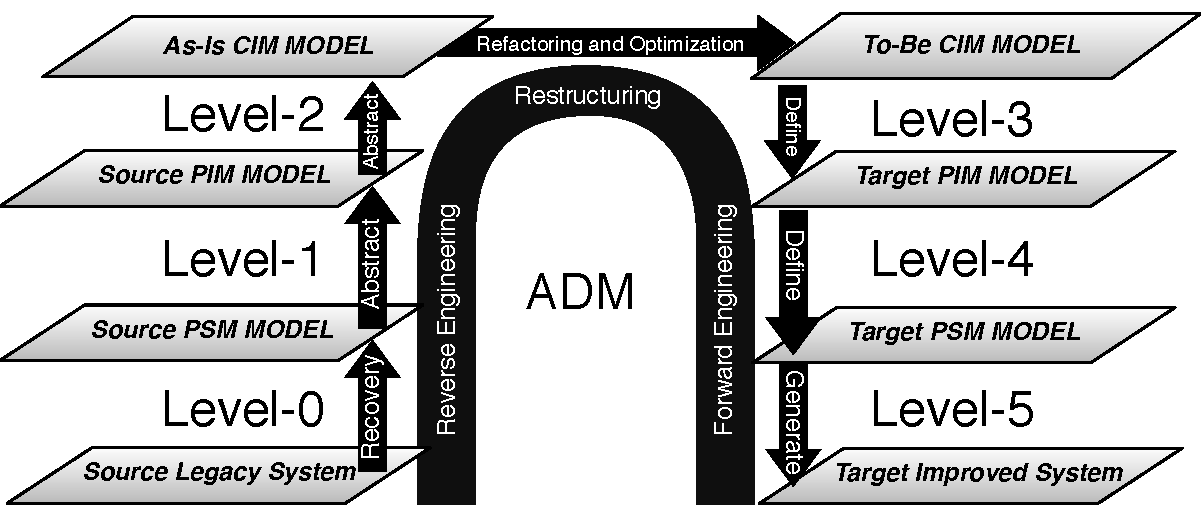
\includegraphics[scale=0.4]{figuras/Fonte_horse_shoe}
\caption{Modernization domain model (Adapted from Ulrich and Newcomb~\cite{Ulrich:2010:IST:1841736})}
\label{horseshoe}
\end{figure}

As can be seen in Figure~\ref{horseshoe} the horseshoe reengineering model has been adapted to ADM and it is nowadays known as horseshoe modernization model. As ADM uses the principles of MDA three kinds of models in the horseshoe are used, they are: (\textit{i}) PIM - \textbf{P}lataform \textbf{I}ndependent \textbf{M}odel which represents a view of the system from the platform independent viewpoint at an intermediate abstraction level, (\textit{ii}) PSM - \textbf{P}lataform \textbf{S}pecific \textbf{M}odel which constitutes a view of the system from the platform specific viewpoint at a low abstraction level, and (\textit{iii}) CIM - \textbf{C}omputational \textbf{I}ndependent \textbf{M}odel that represents a view of the system from the computational independent viewpoint at a high abstraction level. These models are used in the steps of the ADM process, i.e., Reverse Engineering, Restructuring, and Forward Engineering. In the first step, a reverse engineering is performed starting from the artifacts of the legacy system (source code, database, configuration files, etc) and a set of PSM are created. Next, refactoring and restructuring techniques can be applied on these models in order to solve problems found in the legacy system. Therefore, this step consist of a set of transformation from the input model (``as-is'') to obtain a target model (``to-be''). Finally, a forward engineering is carried out and the source code of the modernized target system is generated again. 


In order to perform such steps, ADM introduces several modernization standards: Abstract Syntax Tree Metamodel (ASTM), Knowledge Discovery Metamodel (KDM), Structured Metrics Metamodel (SMM), etc. The next subsections present more information about these standards:


%System Assurance \& Evidence, Software Quality and Business Architecture Standards. Nevertheless, in this paper we are especially interested in KDM, i.e., it is the key cornerstone of ADM and KDM owns a set of metamodel elements whose purpose is to represent implementation level program elements and their associations. The details of KDM are described as follows:

\subsubsection{Abstract Syntax Tree Metamodel - ASTM}

Abstract Syntax Tree Metamodel (ASTM) was established to represent software at a very granular level of procedural logic, data definition, and workflow composition. ASTM can provide this granular level of information to KDM (see Section~\ref{subsec:KDM}) to augment the KDM view of a system. As a standard, ASTM can stand alone and supports tools geared at the complete, functionally equivalent refactoring and transformation of a system from one platform and language environment to a target platform and language environment. ASTM is a model that represent software artifacts using data structures that represent the types of language constructs, its compositional relationships to other language constructs, and a set of direct and derived properties associated with each language construct. The ASTM is derived by analyzing software artifacts and provides a way to create a representation of those software artifacts. 

\begin{figure}[!ht]
\centering
  % Requires \usepackage{graphicx}
  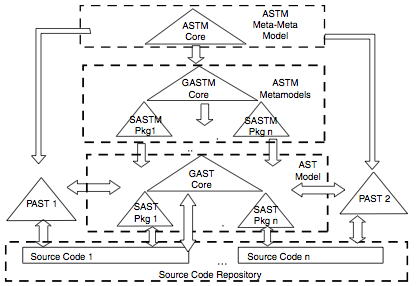
\includegraphics[scale=0.56]{figuras/ASTM}
\caption{ASTM modeling framework}
\label{ASTM}
\end{figure}

ASTM aims to facilitate exchanging software models in standard formats among tools. This ability of exchanging software models between tools is thanks to its attributes, they are: (\textit{i}) ASTM is language and platform independent, but can be extended as needed, (\textit{ii}) ASTM uses XMI formats for tool-based metadata exchange, \textit{iii} Generic Abstract Syntax Tree Metamodel (GASTM) represents a generic set of language modeling elements common across numerous languages. Language Specific Abstract Syntax Tree Metamodel (SASTM) represents particular languages such as Ada, C, FORTRAN, and Java, \textit{iv} Proprietary Abstract Syntax Tree Metamodel (PASTM) expresses ASTs for languages such as Ada, C, COBOL, etc., modeled in formats inconsistent with MOF, the GSATM, or SASTM. Figure~\ref{ASTM} represents the structure of the ASTM, including the SASTM, GASTM, and PASTM.

\subsubsection{Knowledge Discovery Metamodel - KDM}\label{subsec:KDM}

Knowledge Discovery Metamodel (KDM) is the key within set of standards~\cite{1686216}. KDM allows standardized representation of knowledge extracted from legacy systems by means of reverse engineering. KDM provides a common repository structure that makes possible the exchange of information about existing software assets in legacy systems. This information is currently represented and stored independently by heterogeneous tools focused on different software assets~\cite[p.~32]{Ulrich:2010:IST:1841736}. Figure~\ref{kdm} shows each of the varying views of the existing IT architecture represented by the KDM. For example, the build view, depicts system artifacts from a source, executable, and library viewpoint. Other perspectives include design, conceptual, data, and scenario views.

\begin{figure}[!ht]
\centering
  % Requires \usepackage{graphicx}
  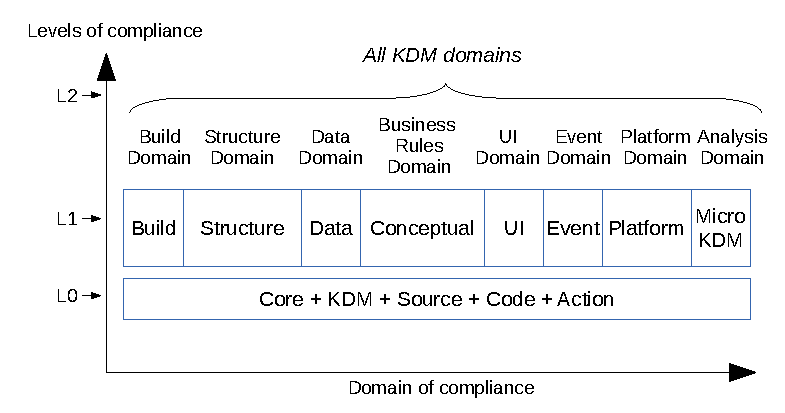
\includegraphics[scale=0.67]{figuras/kdm}
\caption{KDM domains of artifact representation (Adapted from Ulrich and Newcomb~\cite{Ulrich:2010:IST:1841736})}
\label{kdm}
\end{figure}

The Level 0 (L0) encompasses the Infrastructure and Program Elements Layer. Infrastructure Layer consists of the Core, kdm, and Source packages which provide a small common core for all other packages. Program Elements Layer consists of the Code and Action packages providing programming elements such as  data types, data items, classes, procedures, macros, prototypes, templates and captures the low level behavior elements of applications, including detailed control and data flow between statements. The Level 1 (L1) cover the Resource Layer which represents the operational environment of the existing software system. For example, the knowledge related to events and state-transition, the knowledge related to the user interfaces of the existing software system and the knowledge related to persistent data, such as indexed files, relational databases, and other kinds of data storage. The Level 2 (L2) cover the Abstraction Layer which represents domain and application abstractions. 

As we stated earlier, herein we are only interested in the Program Element Layer - more specifically  in the Code Package, which represents the code elements of a program and their associations. Therefore, it is important to dig a little deeper in this metamodel because it is mainly used by our approach in order to identify concerns. 

In a given KDM instance, each instance of the code meta-model element represents some programming language construct, determined by the programming language of the existing software system. Each instance of a code meta-model element corresponds to a certain region of the source code in one of the artifacts of the existing software system. In addition, the Code package consists of $24$ classes  and contains all the abstract elements for modeling the static structure of the source code. However, we are particularly interested in some of them. In Figure~\ref{fig:programLayer} is depicted a chunk of the Code package. It worth to notice that the more important metaclasses used herein are highlighted.

\begin{figure}[!ht]
\centering
  % Requires \usepackage{graphicx}
  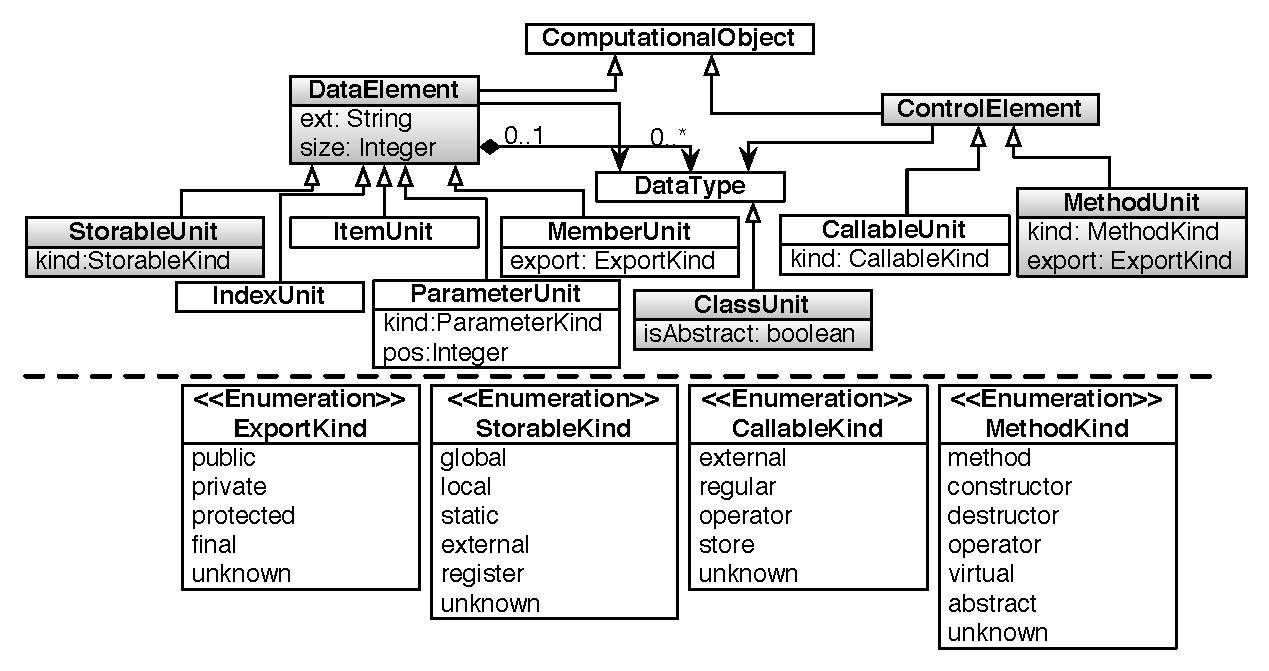
\includegraphics[scale=0.42]{figuras/ProgramLayer}
\caption{Chunk of the Code Package (OMG Group~\cite{OMGADM})}
\label{fig:programLayer}
\end{figure}

As can be seen in Figure~\ref{fig:programLayer} the root metaclass is \textit{ComputationalObject} which has two sub-metaclasses, i.e., \textit{DataElement} and \textit{ControlElement}. The former sub-metaclass, \textit{DataElement}, is a generic modeling element that defines the common properties of several concrete classes that represent the named data items of existing software systems, for example, global and local variables, record files, and formal parameters. \textit{DataElement} has five sub-metaclasses - \textit{StorableUnit}, \textit{IndexUnit}, \textit{ItemUnit}, \textit{ParameterUnit} and \textit{MemberUnit}. \textit{StorableUnit} is a concrete  sub-metaclass of the \textit{StorableElement} meta-class that represents variables of the existing software system. \textit{IndexUnit} class is a concrete subclass of the \textit{DataElement} class that represents an index of an array datatype. Instances of \textit{ItemUnit} class are endpoints of KDM data relations which describes access to complex datatypes. \textit{ParameterUnit} class is a concrete subclass of the \textit{DataElement} class that represents a formal parameter; for example, a formal parameter of a procedure. \textit{MemberUnit} class is a concrete subclass of the \textit{DataElement} class that represents a member of a class type. Finally, the latter, \textit{ControlElement} is a sub-metaclass that contains two sub-metaclasses - \textit{MethodUnit} and \textit{CallableUnit}. \textit{MethodUnit} element represents member functions owned by a \textit{ClassUnit}, including user-defined operators, constructors and destructors. The \textit{CallableUnit} represents a basic stand-alone element that can be called, such as a procedure or a function. As can be seen below the dashed line in Figure~\ref{fig:programLayer} there are also the following enumerations: ``\textit{ExportKind}'', ``\textit{StorableKind}'', ``\textit{CallableKind}'', ``\textit{MethodKind}'', which are sets os literals used as properties of the metaclasses.

\subsubsection{Structured Metrics Metamodel - SMM}

SMM (Structured Metrics Metamodel) provides a standard format to define metrics and to represent the measurement results. The main terms in SMM are measures and measurements. Measures are models which describes a way to calculate properties of software. For measurements can understand models containing results of applications of the metrics.

To apply SMM models in KDM models, a tool is needed to automate the process. The process occurs as illustrated in Figure X, the tool must receive an SMM model and a KDM model as input (KDM represents the software to be measured), then, after the measurements, other SMM model is generated as output and this model contains the results of the process.

There are some advantages in using SMM. It is advantageous because it is a standard, so, metrics defined in accordance with this metamodel can be tested, reused and shared. Furthermore, the use of a standard facilitates the development of compatible tools for automating the measurement process.

The SMM metrics can be of various types; direct, collective, binaries, etc. Direct metrics perform measurements of an index in a model. Collective metrics may measure multiple components and perform an operation with the result, for example; sum, average and others.

%		\subsection{Motivation}
%		Systematic review studies belong to Evidence-Based Software Engineering (EBSE) paradigm [36]. They provide new, empirical and systematic methods of research. Although several studies have been reported in the broader context of Architecture Driven Modernization (ADM)~\cite{PerezCastillo20121370, SMR:SMR582, FuentesFernandez2012247, PrezCastillo2011519}, to the best of our knowledge any systematic review has been conducted in this field. As for the fact that various types of research have appeared addressing diversifying focus areas related to the topic of modernization of legacy system by means of ADM, we claim the need for a more systematic investigation of this topic. As result, this paper is meant to furnish to ADM through a systematic review and evidence-based approach. Also we argue that this paper may help researchers in the field of modernization of legacy systems, once the paper provides an overview of the current state-of-the-art of the ADM. Furthermore, it may serve as a first step towards more thorough examination of the topics addressed in it with the help of systematic literature reviews.
	

\section{The Systematic Review}\label{method}
	This study has been undertaken as a systematic review based on the guidelines proposed by Kitchenham and Brereton~\cite{Kitchenham}. According to them, in order to conduct a systematic review, it is advisable to follow three main phases: (\textit{i}) planning the review, (\textit{ii}) conducting the review and (\textit{iii}) reporting the review. %In Figure~\ref{process_systematic_review} depicts these three phases that we carried out herein. 
Furthermore, in this paper we have used Visual Text Mining (VTM) technique to support the studies selection~\cite{Malheiros:2007}. VTM uses text mining algorithms and methods combined with interactive visualisations. Therefore, it can help the user making sense of a collection of primary studies, without actually reading all of them. In this case the studies were reading partially or full. The following sections present details on how each phase was carried out.

%\begin{figure}[!h]
%\centering
  % Requires \usepackage{graphicx}
%  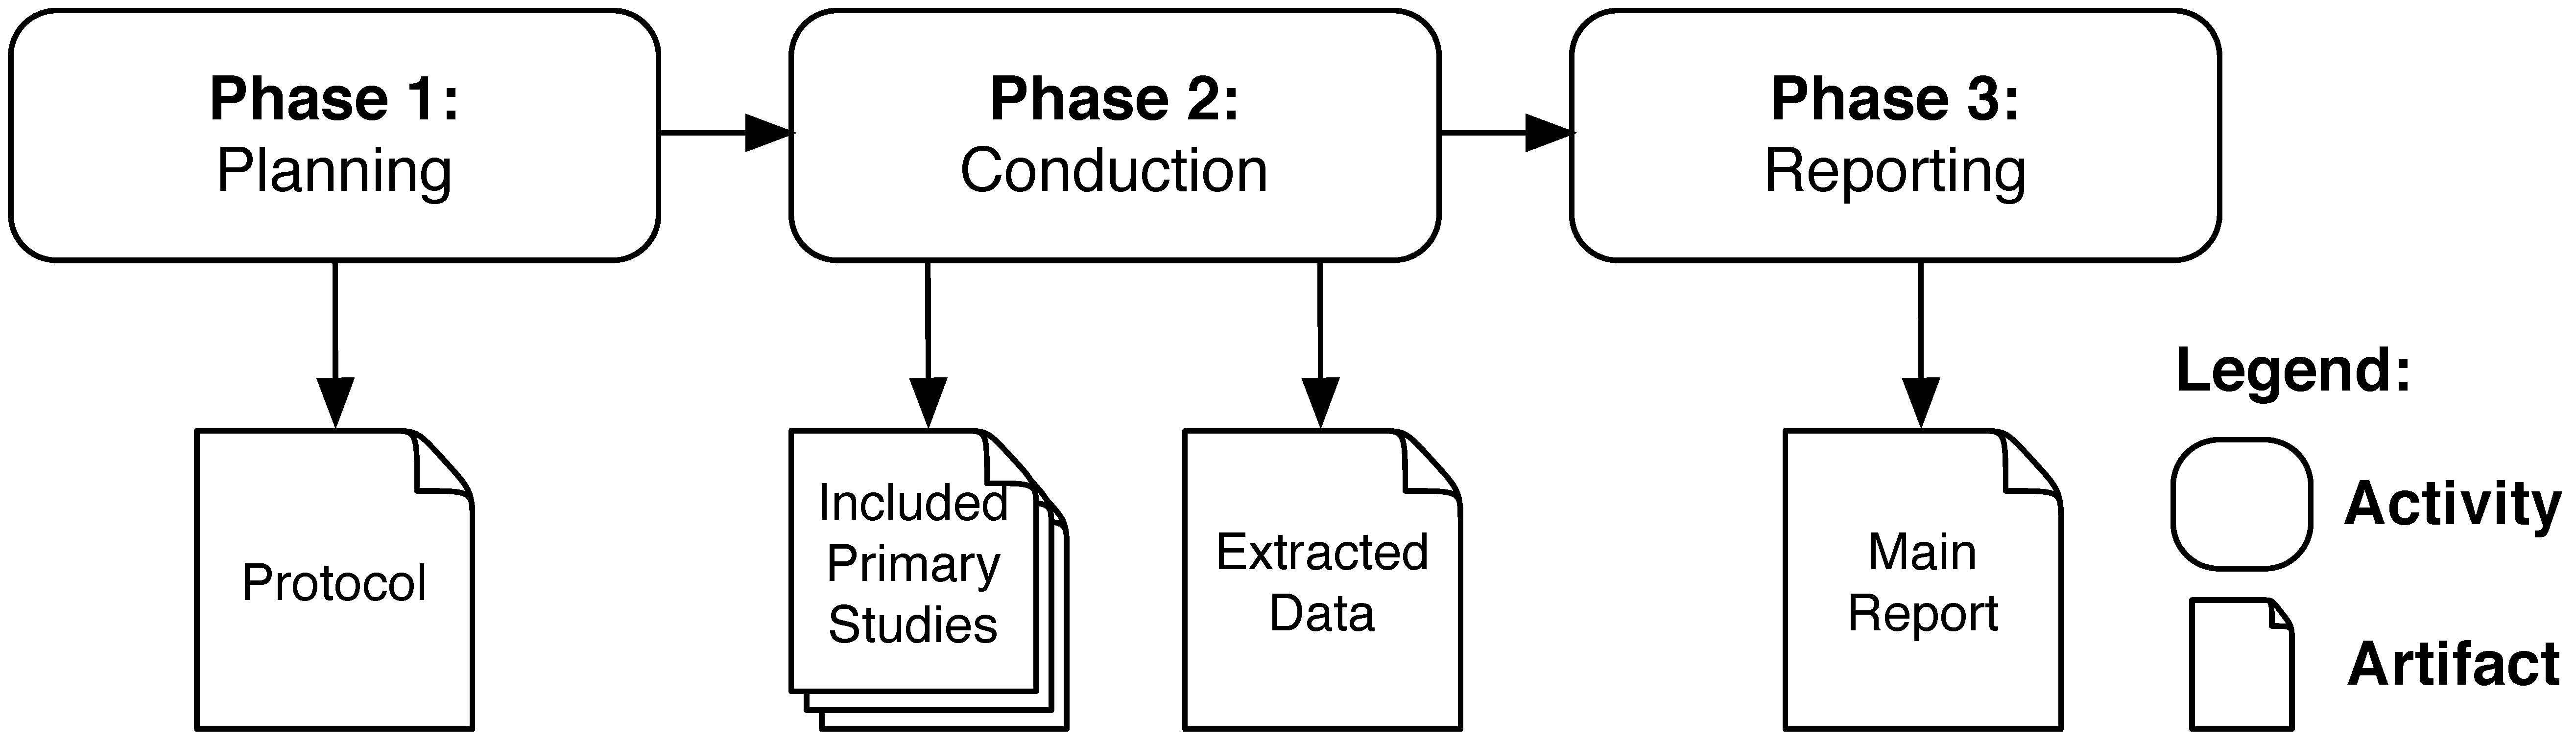
\includegraphics[scale=0.09]{figuras/process}
%\caption{Systematic review process (Adapted from Kitchenham~\cite{Kitchenham}).}
%\label{process_systematic_review}
%\end{figure} 
	\subsection{Planning the Systematic Review\label{planning}}
		In this phase we defined the review protocol. This protocol contains: (\textit{i}) the research questions, (\textit{ii}) the search strategy, (\textit{iii}) the inclusion and exclusion criteria and (\textit{iv}) the data extraction and synthesis method.

%Research questions must embody the review study purpose. Moreover, these questions reflect the general scope of the review study. The scope is comprised of population (i.e., population group observed by the intervention), intervention (i.e., what is going to be observed in the context of the planned review study), and outcomes of relevance (i.e., the results of the intervention). Furthermore, during the conduction of this step, it was also necessary to establish the scope of the review study. According to the systematic review process~\cite{Kitchenham}, the scope has to be established using the PICO criteria. Thus, herein our \textbf{Population} is published scientific literature reporting on the use of Architecture-Driven Modernization and its metamodels. The \textbf{Intervention} is published scientific literature interested with Architecture-Driven Modernization and its metamodels. The \textbf{Comparison} is not applied herein. Finally, the \textbf{Outcomes of relevance} is an overview of the studies that have been conducted in the field of Architecture-Driven Modernization and its metamodels, emphasizing primary studies that report on the process used in the research area, from observing such an aggregated data set, we also intend to provide insight into the frequencies of publication over time to inspect trends.   

%\begin{itemize}

%\item \textbf{Population:} published scientific literature reporting on some existing mining techniques for crosscutting concern.

%\item \textbf{Intervention:} published scientific literature concerned with mining techniques for crosscutting concern. Furthermore, we also aim at determining which techniques are the most used within academic settings.

%\item \textbf{Comparison:} No applied herein.

%\item \textbf{Outcomes of relevance:} an overview of the studies that have been conducted in the field of crosscutting concern mining, emphasizing primary studies that report on the techniques used in the research area. From observing such an aggregated data set we also intend to provide insight into the frequencies of publication over time to inspect trends.

%\end{itemize} 

%Como ADM esta sendo aplicada na literatura para auxiliar a modernizacao de sistemas legados

As described before, the objective of this review is to find out \textbf{how ADM has been applied in the literature to assist engineers during the process of modernization of legacy systems}. In order to achieve such objective we worked out five research questions. The questions are: \textbf{RQ$_1$:} What are the focus area most discussed and least discussed in the literature regarding the ADM? Moreover, what types of contributions have been presented so far?; \textbf{RQ$_2$:} Given the ADM's standards metamodels, which one has been more used in the literature? In addition, given the identified metamodel, what are the packages most and least used?; \textbf{RQ$_3$:} Which research types have been employed into the field herein?; \textbf{RQ$_4$:} Which are the existing tool support for ADM? Moreover, how the tools perform the identification of what needs to be modernized?

%\begin{description}

%\item[\textbf{RQ$_1$:}] What are the focus area most discussed and least discussed in the literature regarding the ADM? Moreover, what types of contributions have been presented so far?

%\item[\textbf{RQ$_2$:}] Given the ADM's standards metamodels, which one has been more used in the literature? In addition, given the identified metamodel, what are the packages most and least used?

%\item[\textbf{RQ$_3$:}] Which research types have been employed into the field herein?

%\item[\textbf{RQ$_4$:}] Which avenues are often used to publish research related to ADM?

%\item[\textbf{RQ$_5$:}] Which are the existing tool support for ADM? Moreover, how the tools perform the identification of what needs to be modernized?



%\item[\textbf{RQ$_4$:}] Given a set of concerns, which are the most indicated techniques for performing the mining?

%\item[\textbf{RQ$_5$:}] How can someone combine the techniques for improving the precision and recall metrics?

%\item[\textbf{RQ$_3$:}]  Considering the techniques that we found, which ones have automated support?

%\end{description}

To address \textbf{RQ$_1$}, we read all primary studies in order to identify the focus area of each study. Next, we arrange all studies according to the focus area. Whether any kind of disagreement related to the focus area that the article meets, it was marked and was discussed with everyone involved in the review in order to clarify which topic it belongs. With respect to \textbf{RQ$_2$}, we also read all primary studies and identified which metamodel was used in the study. With respect to \textbf{RQ$_3$}, we used and adapted the scheme proposed by Wieringa et al~\cite{Wieringa:2005:REP:1107677.1107683} in order to classify each primary studies into a research type, see Section~\ref{research_type}. Finally, to address \textbf{RQ$_4$} we read all primary studies in order to identifiy the tools used to modernize the legacy systems. %Next, we arrange the identified tools according to the focus area. 


Afterwards, we have defined the search string and chosen the electronic databases. The search string was created based upon a set of keywords. A sophisticated search string was constructed using boolean operators i.e., \textit{AND} and \textit{OR}. Figure~\ref{search_string} shows the search string elaborated. The search have encompassed electronic databases which are deemed as the most relevant scientific sources~\cite{Dyba} and therefore likely to contain important primary studies. We have used the search string on the following electronic databases: \textit{ACM}, \textit{IEEEXPLORE}, \textit{Scopus}, \textit{Web of Science} and \textit{Engeneering Village}. Note that since the features provided by various databases as well as the exact syntax of search strings to be applied vary from one database to other, the string given in Figure~\ref{search_string} was actually used to construct a semantically equivalent string specific to each database.

%Furthermore, no limits were placed on date of publication with a view to not restrict the review study scope. %Aimed at keeping track of the selected papers, we used JabRef\footnote{http://jabref.sourceforge.net/}, an open source system for bibliography reference management. 

\begin{figure}[!h]
\centering
  % Requires \usepackage{graphicx}
  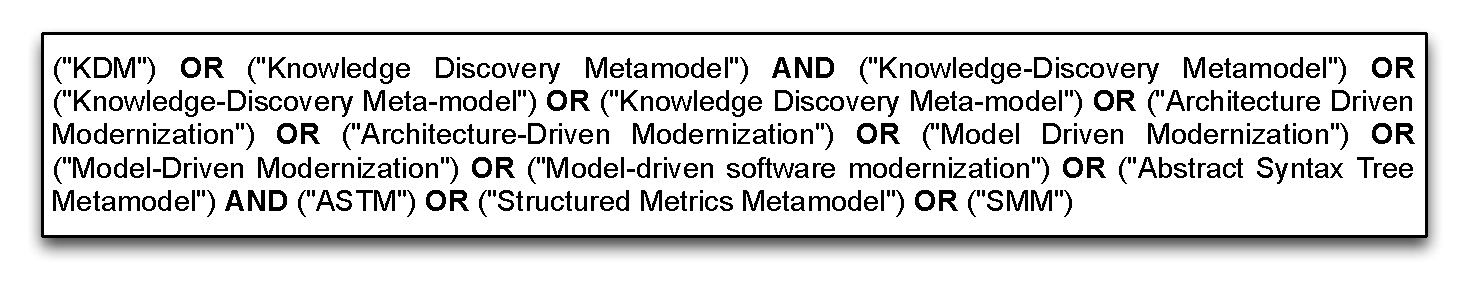
\includegraphics[scale=0.35]{figuras/SearchStringADM}
\caption{Search String.}
\label{search_string}
\end{figure} 

Then, in order to determine which primary studies are relevant to answer our research questions, we have applied a set of inclusion and exclusion criteria. Inclusion criteria devised and applied are: (\textit{i}) \textbf{The primary study presents at least one solution of modernization by means of ADM} - (\textit{ii}) \textbf{Studies that explicitly present an ADM approach} - (\textit{iii}) \textbf{The primary study presents at least one type of evaluation technique for ADM}.  

%\begin{enumerate}[(a)]%for small alpha-characters within brackets.
%\item \textbf{The primary study presents at least one solution of modernization by means of ADM:} the paper provides evidences that the ADM assists the software engineer during the modernization/refactoring of legacy system.

%\item \textbf{Studies that explicitly present an ADM approach:} the paper provides an approach to assist the software engineer to modernize the legacy system.

%\item \textbf{The primary study presents at least one type of evaluation technique for ADM:} without the results of the evaluation we would not be able to make comparisons desired. In other words, the paper must clearly present which assessment techniques have been employed to evaluate the ADM process, i.e., case study, experiment, survey, etc.

%\end{enumerate}

Not all of these criteria must be present for every primary study. However, at least the former, i.e., (a), must be present. If all criteria were mandatory, the number of selected techniques would decrease significantly.

Exclusion criteria devised and applied are: (\textit{i}) \textbf{Papers which mentioned ADM and its metamodels in the abstract only} - (\textit{ii}) \textbf{Papers that present only recommendations, guidelines or principles} - (\textit{iii}) \textbf{Introductory papers for books and workshops} - (\textit{iv}) \textbf{The primary study is a short paper} - and (\textit{v}) \textbf{Papers from industrial conferences, and non English publications}. 
%\begin{enumerate}[(a)]

%\item \textbf{Papers which mentioned ADM and its metamodels in the abstract only:} this was required because we found many studies that mentioned ADM and its metamodels in their opening sentences as a principal concept, however, the studies did not really address it.

%\item \textbf{Papers that present only recommendations, guidelines or principles:} usually this kind of papers do not present practical approach to modernize legacy systems.

%\item \textbf{Introductory papers for books and workshops.}

%\item \textbf{The primary study is a short paper:} papers with two pages or less were not considered herein, since we considered that this kind of study do not own sufficient information.

%\item \textbf{Papers from industrial conferences, and non English publications.}
 
%\end{enumerate}

% \textbf{IC$_1$:} the primary study presents at least one mining technique for crosscutting concern and \textbf{IC$_2$:} the primary study presents at least one type of evaluation technique for crosscutting concern. And the following exclusion criteria: \textbf{EC$_1$:} the primary study presents data mining technique, however, such technique is applied to databases and not for crosscutting concern mining and \textbf{EC$_2$:} the primary study is a short paper (papers with twos pages or less).

%\begin{description}

%\item[\textbf{IC$_1$:}] The primary study presents at least one mining technique for crosscutting concern

%\item[\textbf{IC$_2$:}] The primary study presents at least one type of evaluation technique for crosscutting concern.

%\end{description}

%and the following exclusion criteria:

%\begin{description}

%\item[\textbf{EC$_1$:}] The primary study is not about mining techniques for crosscutting concern.

%\item[\textbf{EC$_2$:}] The primary study presents data mining technique. However, such technique is applied to databases and not for crosscutting concern mining.

%\item[\textbf{EC$_3$:}] The primary study is not available in an electronic format.

%\item[\textbf{EC$_3$:}] The primary study is a short paper (papers with twos pages or less).

%\item[\textbf{EC$_5$:}] The primary study is written neither english nor portuguese.

%\end{description}

We devised data extraction forms to accurately record the information obtained by the researchers from the primary studies. The form for data extraction provides some standard information, such as (\textit{i}) a brief of the primary study, highlighting where ADM and its metamodels are used, (\textit{ii}) date of data extraction, (\textit{iii}) title, authors, journal, publication details and (\textit{iv}) a list of each conclusion and statement encountered for each question. 

During the extraction process, the data of each primary study were independently gathered by three reviewers. The review was performed in August, 2013 by two M.Sc. and a Ph.D. student; the achieved results were crossed and then validated. All the results of the search process are documented in the web material\footnote{http://tinyurl.com/99spmaz}. Therefore, it is clear to others how thorough the search was, and how they can find the same documents.

	\subsection{Conducting the Systematic Review\label{conducting}}
		%In Figure 2~\ref{process} the three steps of the conduction phase. As can be seen, in Step 1, we identified primary studies in the digital libraries. The digital libraries Scopus has returned more primary studies than the others(262), i.e., IEEE, ACM and Springer have returned 215, 202 and 127, respectively. Possibly, this came about because this digital library indexes studies of others libraries, such as IEEE and Springer. Summing up, we have gotten 802 primary studies in the Step 1. In the Step 2 we have selected the primary studies by means of reading the titles and abstracts and the application of the inclusion and exclusion criteria. As a result, we have gotten a total of 124 primary studies that were read entirely, so the upshot obtained in the Step 3 were 62. Among these 62 primary studies we have identified 18 mining techniques for crosscutting concern. Therefore, each included primary study was assigned to one or more techniques.
%
%\begin{figure}[!h]
%\centering
%  % Requires \usepackage{graphicx}
%  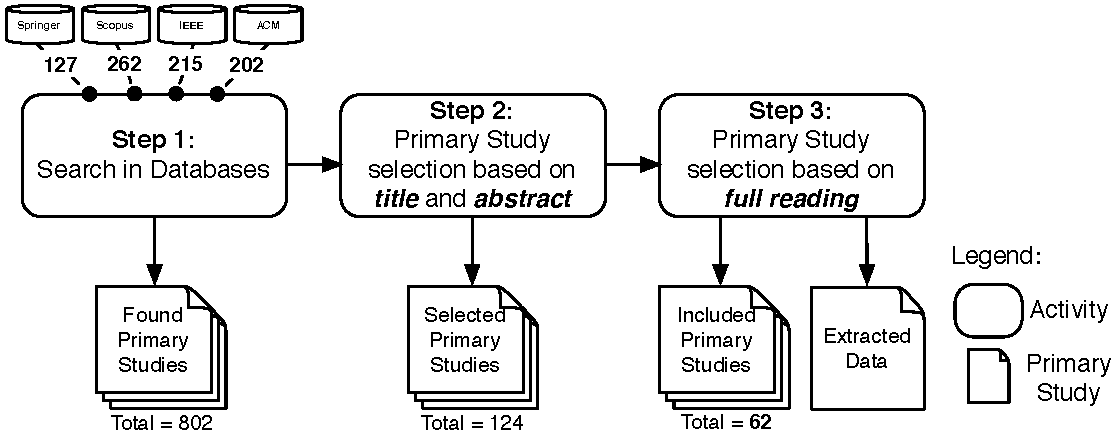
\includegraphics[scale=0.4]{figuras/process_conducted}
%\caption{Papers retrieved from each electronic database, total of candidate studies and the final set.}
%\label{process}
%\end{figure} 

In this phase, firstly we identified primary studies in the digital libraries, i.e., IEEE, ACM, Scopus, Web of Science and Engeneering Village. We applied the search string given in Figure~\ref{search_string}. %Thus, an overview of results acquired from these digital libraries is depicted in Table~\ref{result_digital}.

%\begin{table}[!h]
%\centering
%\caption{Overview of search results.}
%\begin{tabular}{|c|c|}
%\hline 
%\cellcolor{gray}Digital Libraries & \cellcolor{gray}Number\tabularnewline
%\hline 
%\hline 
%Scopus & 150\tabularnewline
%\hline 
%ACM & 51\tabularnewline
%\hline 
%Engeneering Village & 30\tabularnewline
%\hline 
%Web of Science & 17\tabularnewline
%\hline 
%IEEE & 11\tabularnewline
%\hline 
%\cellcolor{gray!25}Total & \cellcolor{gray!25}259\tabularnewline
%\hline 
%\cellcolor{gray!25}Candidates & \cellcolor{gray!25}82\tabularnewline
%\hline 
%\cellcolor{gray!25}Final set & \cellcolor{gray!25}30\tabularnewline
%\hline 
%\end{tabular}
%\label{result_digital}
%\end{table} 


%As can be seen in Table~\ref{result_digital} 
The digital libraries Scopus has returned more primary studies than the others (150), ACM, Engeneering Village, Web of Science and IEEE returned 51, 30, 17 and 11, respectively. Possibly, this came about because Scopus indexes studies of others libraries, such as IEEE and ACM. Summing up, we have gotten 259 primary studies. After performing automatic search, we excluded the duplicate publications. If a primary study was found in more than once, we selected the most recent and detailed version of the paper. Afterwards, we selected the primary studies by means of reading the titles and abstracts and the application of the inclusion and exclusion criteria. At this stage, we also narrowed down the categories of publications to some extent by excluding non-peer reviewed publications, in order to ensure a level of quality as well as to avoid redundancy in contributions. As a result, we have gotten a total of 82 primary studies that were read entirely, so the upshot obtained were 30 studies. A total of 229 studies were excluded either due to their limited relevance or meeting one of the other exclusion criterions (see Section~\ref{planning}).

We applied the classification schemes proposed by Petersen et al.~\cite{Petersen:2008:SMS:2227115.2227123} and classified the publications into categories from three perspectives, as follows: (\textit{i}) focus area, (\textit{ii}) contribution type and (\textit{iii}) research type. We chose this classification scheme because it is highly used in secondary study, i.e., papers which describe systematic review and systematic mapping~\cite{Mehmood:2013:AMC:2400747.2401009}. %Although, this classification schemes has been proposed to be applied during a systematic mapping, we claim that it can be used during the systematic review process as well. 
Thus, the aforementioned categories were adapted to specifics of our systematic study. The resultant classification schemes are as follows:

\subsubsection{Focus Area}

We have used the keywording method described in~\cite{Petersen:2008:SMS:2227115.2227123} to identify the focus area of the studies identified. As result we got four ones - a brief description of each focus area follows: (\textit{i}) \textbf{Approaches to modernize legacy systems to another platform/architecture (SOA, change programming language, web $2.0$, mobile, etc):} This focus area is related to primary studies which describe process, method or approach that uses ADM and its metamodels to modernize legacy systems either to another platform  or architecture; (\textit{ii}) \textbf{Business Knowledge Extraction:} Describes primaries studies which address process, method or approach to extract business process of a legacy system; (\textit{iii}) \textbf{Extension of ADM's Metamodels:} This focus area represents primary studies which report an approach, method or process to extend one of the ADM's metamodels, e.g., extension of KDM, SMM, ASTM, etc; and (\textit{iv}) \textbf{Applicability:} This category includes papers that mainly focus on reporting evidence related to applying ADM and its metamodels in practice. In other words, papers which enable researchers and practitioners to get a better understanding of ADM and its metamodels, e.g., papers that show how to use the metamodels (KDM, SMM and ASTM) and provide a basis for the further research, etc.

%\begin{itemize}

%\item \textbf{Approaches to modernize legacy systems to another platform/architecture (SOA, change programming language, web $2.0$, mobile, etc):} This focus area is related to primary studies which describe process, method or approach that uses ADM and its metamodels to modernize legacy systems either to another platform  or architecture.

%\item \textbf{Business Knowledge Extraction:} Describes primaries studies which address process, method or approach to extract business process of a legacy system.

%\item \textbf{Extension of ADM's Metamodels:} This focus area represents primary studies which report an approach, method or process to extend one of the ADM's metamodels, e.g., extension of KDM, SMM, ASTM, etc. 

%\item \textbf{Applicability:} This category includes papers that mainly focus on reporting evidence related to applying ADM and its metamodels in practice. In other words, papers which enable researchers and practitioners to get a better understanding of ADM and its metamodels, e.g., papers that show how to use the metamodels (KDM, SMM and ASTM) and provide a basis for the further research, etc.

%\end{itemize}


\subsubsection{Contribution Type}


During the reading of the primary studies was possible to identify a set of contribution type related to ADM and its metamodels. More precisely we identified five contribution type: (\textit{i}) \textbf{Tool:} This contribution type refers to the primary studies found that focus on providing tool in order to support the modernization of legacy system by using ADM and its metamodels, i.e., either in the form of a prototype or a tool that can be integrated with existing environment; (\textit{ii}) \textbf{Process:} Similarly, it refers to contributions which specifically describe a process to assist the modernization of legacy system by means of ADM and its metamodels; (\textit{iii}) \textbf{Model Transformation:} It refers to contributions which specifically describe transformation among ADM's metamodels, e.g., primary studies that describe the use of language transformation such as either Query/Views/Transformations (QVT)\footnote{http://www.omg.org/spec/QVT/1.1/} or ATL Transformation Language (ATL)\footnote{www.eclipse.org/atl/}; (\textit{iv}) \textbf{Metamodel:} This contribution type describes primary studies which either created or extended the ADM's metamodels to deal with a specific problem, for instance, providing a KDM light-weight extension in order to either represent the aspect oriented paradigm or supports a component-oriented decomposition; and (\textit{v}) \textbf{Metrics:} This is type of contributions focus on proposing or applying metrics to effectiveness of ADM and its metamodels.

%\begin{itemize}

%\item \textbf{Tool:} This contribution type refers to the primary studies found that focus on providing tool in order to support the modernization of legacy system by using ADM and its metamodels, i.e., either in the form of a prototype or a tool that can be integrated with existing environment.



%\item \textbf{Process:} Similarly, it refers to contributions which specifically describe a process to assist the modernization of legacy system by means of ADM and its metamodels.

%\item \textbf{Model Transformation:} It refers to contributions which specifically describe transformation among ADM's metamodels, e.g., primary studies that describe the use of language transformation such as either Query/Views/Transformations (QVT)\footnote{http://www.omg.org/spec/QVT/1.1/} or ATL Transformation Language (ATL)\footnote{www.eclipse.org/atl/}. 

%\item \textbf{Metamodel:} This contribution type describes primary studies which either created or extended the ADM's metamodels to deal with a specific problem, for instance, providing a KDM light-weight extension in order to either represent the aspect oriented paradigm or supports a component-oriented decomposition.


%\item \textbf{Metrics:} This is type of contributions focus on proposing or applying metrics to effectiveness of ADM and its metamodels

%\end{itemize}

\subsubsection{Research Type}\label{research_type}

The research type reflects the research approach used in the primary study. Therefore, we used and adapted the scheme proposed by Wieringa et al~\cite{Wieringa:2005:REP:1107677.1107683}. A brief description of research types are as follows: (\textit{i}) \textbf{Validation research:} The main purpose of validation research is to examine a solution proposal that has not yet been practically applied. Validation research is conducted in a systematic way and may present any of these: prototypes,mathematical analysis, etc; (\textit{ii}) \textbf{Evaluation research:} In contrast to validation research, evaluation research aims at examining a solution that has already been practically applied. It investigates the practical implementation of solution and usually presents results using field studies, experiments, or case studies, etc; (\textit{iii}) \textbf{Conceptual proposal:} A conceptual proposal presents an arrangement to see things that already exist, in a novel way. However it does not precisely solve a particular problem. Conceptual proposals may include taxonomies, theoretical frameworks, etc; (\textit{iv}) \textbf{Experience paper:} An experience paper reports on personal experience of the author from one or more real life projects. It usually elaborates on what was accomplished in the project as well as how it was actually done; and (\textit{v}) \textbf{Opinion paper:} Opinion papers report on personal opinion of the author on suitability or unsuitability of a specific technique or tool. Similarly, these are sometimes used to share personal opinion describing as to how some technique or tool should have been developed, etc.

%\begin{itemize}
 
%\item \textbf{Validation research:} The main purpose of validation research is to examine a solution proposal that has not yet been practically applied. Validation research is conducted in a systematic way and may present any of these: prototypes,mathematical analysis, etc. 

%\item \textbf{Evaluation research:} In contrast to validation research, evaluation research aims at examining a solution that has already been practically applied. It investigates the practical implementation of solution and usually presents results using field studies, experiments, or case studies, etc.

%\item \textbf{Conceptual proposal:} A conceptual proposal presents an arrangement to see things that already exist, in a novel way. However it does not precisely solve a particular problem. Conceptual proposals may include taxonomies, theoretical frameworks, etc.

%\item \textbf{Experience paper:} An experience paper reports on personal experience of the author from one or more real life projects. It usually elaborates on what was accomplished in the project as well as how it was actually done.

%\item \textbf{Opinion paper:} Opinion papers report on personal opinion of the author on suitability or unsuitability of a specific technique or tool. Similarly, these are sometimes used to share personal opinion describing as to how some technique or tool should have been developed, etc.

%\end{itemize}
	\subsection{Validation\label{validation}}
		In validation phase an approach that uses VTM technique and the associated tool - Projection Explorer (PEx) - were applied to support the inclusion and exclusion decisions~\cite{Malheiros:2007}. %PEx adopts a two-dimensional visual representation, known as document map, where each document is mapped to a graphical element on the plane, usually a circle (point), with points relative positions reflecting similarity relationships between the contents of the documents they represent. Thereby, on the layout, similar documents are put close to one another, while dissimilar ones are supposed to be positioned far apart.

\begin{figure}[!h]
\centering
  % Requires \usepackage{graphicx}
 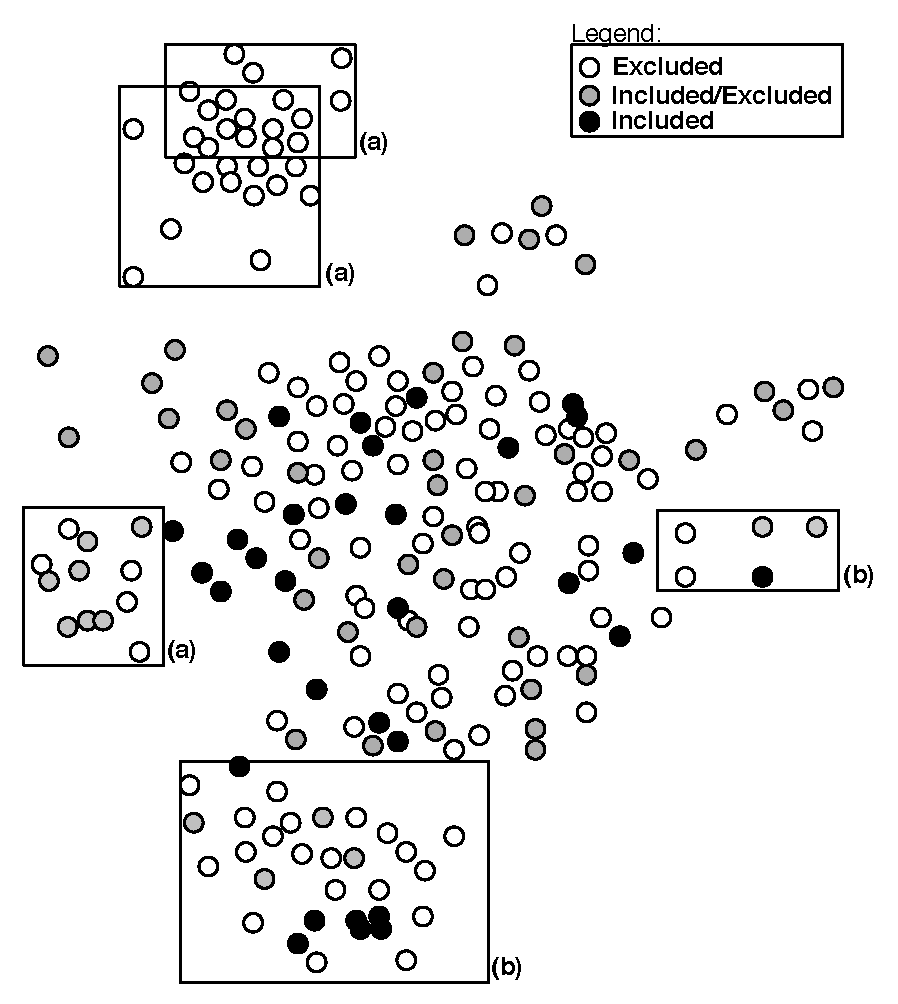
\includegraphics[scale=0.40]{figuras/validation2}
\caption{Document map colored with the history of the inclusions and exclusions of the studies.}
\label{fig:validation}
\end{figure} 

Figure~\ref{fig:validation} presents a document map generated using PEx. This map is composed of 259 primary studies analysed in this review, highlighting them using different shades of gray to differentiate in which of the stages a study was removed from the review. White points are studies excluded in first stage, gray points are the studies excluded in second stage and the black points are the included. The exploration of a document map is conducted in two steps: (\textit{i}) firstly, a clustering algorithm is applied to the document map, creating groups of highly related documents; (\textit{ii}) secondly, the resulting clusters are analysed in terms of:~\textbf{Pure Clusters} - all documents belonging to a cluster have the same classification (all included or excluded, regardless of exclusion stage). Normally, in this case do not need to be reviewed; and~\textbf{Mixed Clusters} - which represent documents with different classification on the same cluster. These cases are hints to the reviewer, and the estuaries grouped should be reviewed following the traditional method. To facility the visualisation, in Figure~\ref{fig:validation} just five clusters generated by PEx are depicted. Examples of pure clusters (all excluded) are identified in Figure~\ref{fig:validation} using label ``(a)'' and therefore do not needed to be reviewed. Mixed clusters (clusters containing black (included) and white or gray (excluded) studies) are identified using label ``(b)'' and they were reviewed by the authors of this paper. At the end, we kept the initial classifications conducted manually, but this technique contributed to a review of studies that could have been wrongly excluded or included previously.  

	
	\subsection{Reporting the Systematic Review\label{reporting}}
		

The focus of this section is to present the broad overview of research within ADM and its metamodels we have acquired after conducting the systematic review. Moreover, we used information drawn from this overview to answer this review study's research questions. Notice that we present our results in two dimensions: (\textit{i}) what are the focus area most discussed and least discussed in the literature regarding the ADM and its metamodels, contribution types (\textbf{RQ$_1$}), research type (\textbf{RQ$_3$}), among metamodels which is more used to assist the modernization (\textbf{RQ$_2$}), the existing tool support for ADM (\textbf{RQ$_4$}).

\begin{figure*}[t]
\centering
  % Requires \usepackage{graphicx}
  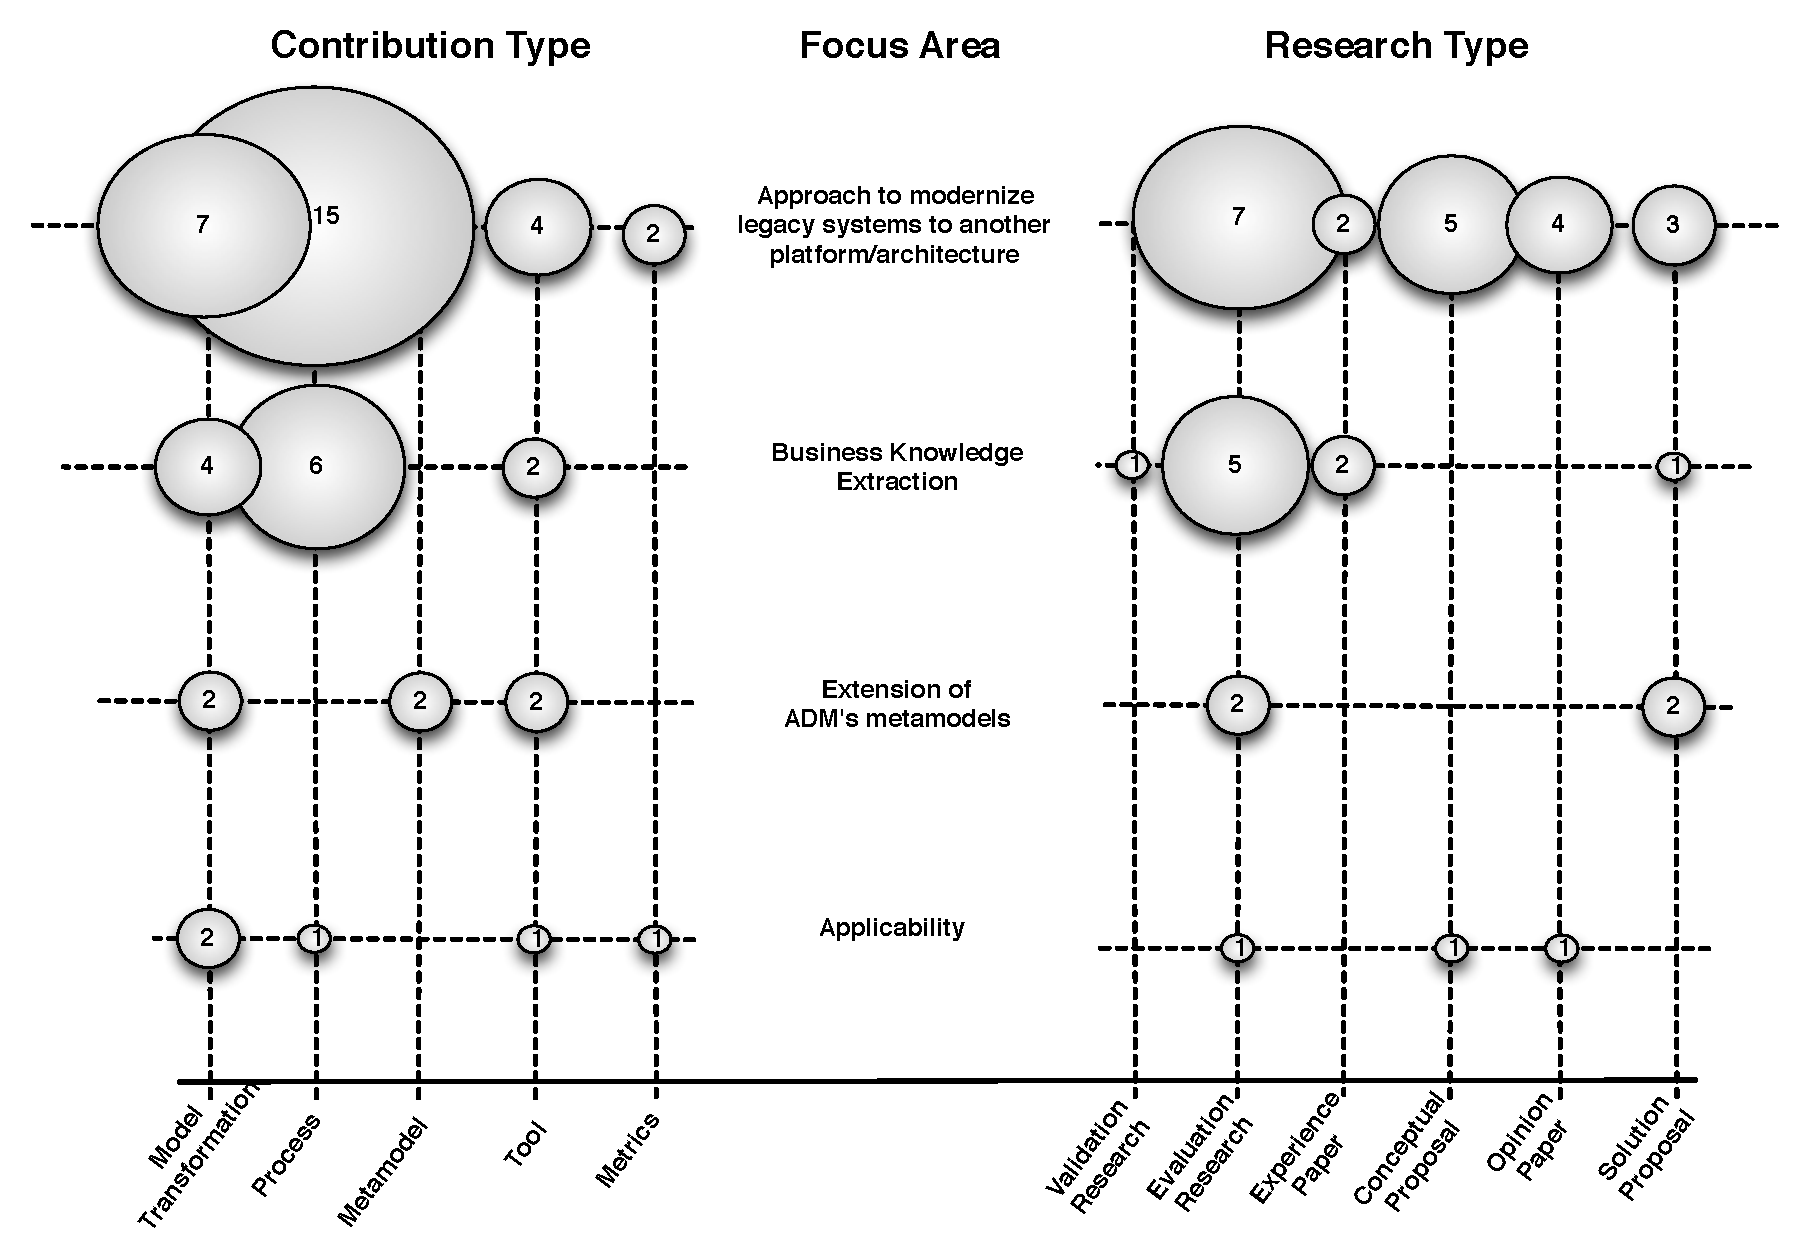
\includegraphics[width=17.5cm, height=7.4cm]{figuras/MapaNOVO3}
\caption{Map of research focus on ADM and its metamodels.}
\label{map}
\end{figure*} 


Aiming to show a part of the first dimension of our results and also the frequencies of all publication related to ADM and its metamodels we plotted a bubble plot, which is depicted in Figure~\ref{map}. Bubble plots are essentially two x-y scatter plots with bubbles in category intersections. The size of each bubble is determined by the number of primary studies that have been classified as belonging to the categories corresponding to the bubble coordinates. This visual summary provides a bird's-eye view that enables one to pinpoint which categories have been emphasized in past research along with gaps and opportunities for future research.

In Figure~\ref{map} the facets we used for organizing the map are the \textbf{contribution type}, \textbf{focus area} and \textbf{research type}. It is worth highlighting that certain primary studies were grouped in more than one category, affecting the frequency count; i.e., the sum of the frequencies shown in each facet can be greater than the total of selected studies presented earlier (30).

 It is fairly evident from observing Figure~\ref{map} that majority of research papers are specifically dedicated for providing \textbf{Process} to assist software engineer during the modernization of legacy system to another platform/architecture. Similarly, \textbf{Model transformation} and \textbf{Tool} (to assist ADM's process) are also another field which have been researched. Maybe this came about once the majority of the primary studies found which describe a process to assist the modernization of legacy systems usually propose a set of model transformation and a semi-automatic tool or a fully-automatic one. In contrast, the contribution type with less studies are \textbf{Metamodel} and \textbf{Metrics}. Thus, it is argued that primary studies that describe process to assist the modernization of legacy systems by means of ADM and its metamodels, papers which show a set of rules to be applied during model transformation among the ADM's metamodels (KDM, SMM and ASTM), and papers which devise tools to assist ADM's process are evidence clusters (i.e., where there may be scope for more complete literature reviews to be undertaken), whereas metamodels (i.e., papers that explain how to extend ADM's metamodels) and metrics (i.e., papers which describe how to apply metrics in ADM's metamodel) can be regarded as gaps (i.e., where new or better primary studies are required). In other words, \textbf{Process} to assist software engineer during the modernization of legacy system to another platform/architecture, \textbf{Model transformation} and \textbf{Tool} have been covered by over 43\%, 29\% and 17\%, respectively of the current research (see Figure~\ref{fig:bar}). On the other hand, \textbf{Metamodel} and \textbf{Metrics} have been addressed by a very small number of publications i.e., 3.92\% and 5.88\%, respectively (see Figure~\ref{fig:bar}).   %pieEvaluation

%\begin{figure*}[!h]
% 
%    \subfloat[Frequency of studies in each category.\label{fig:bar}]{
%     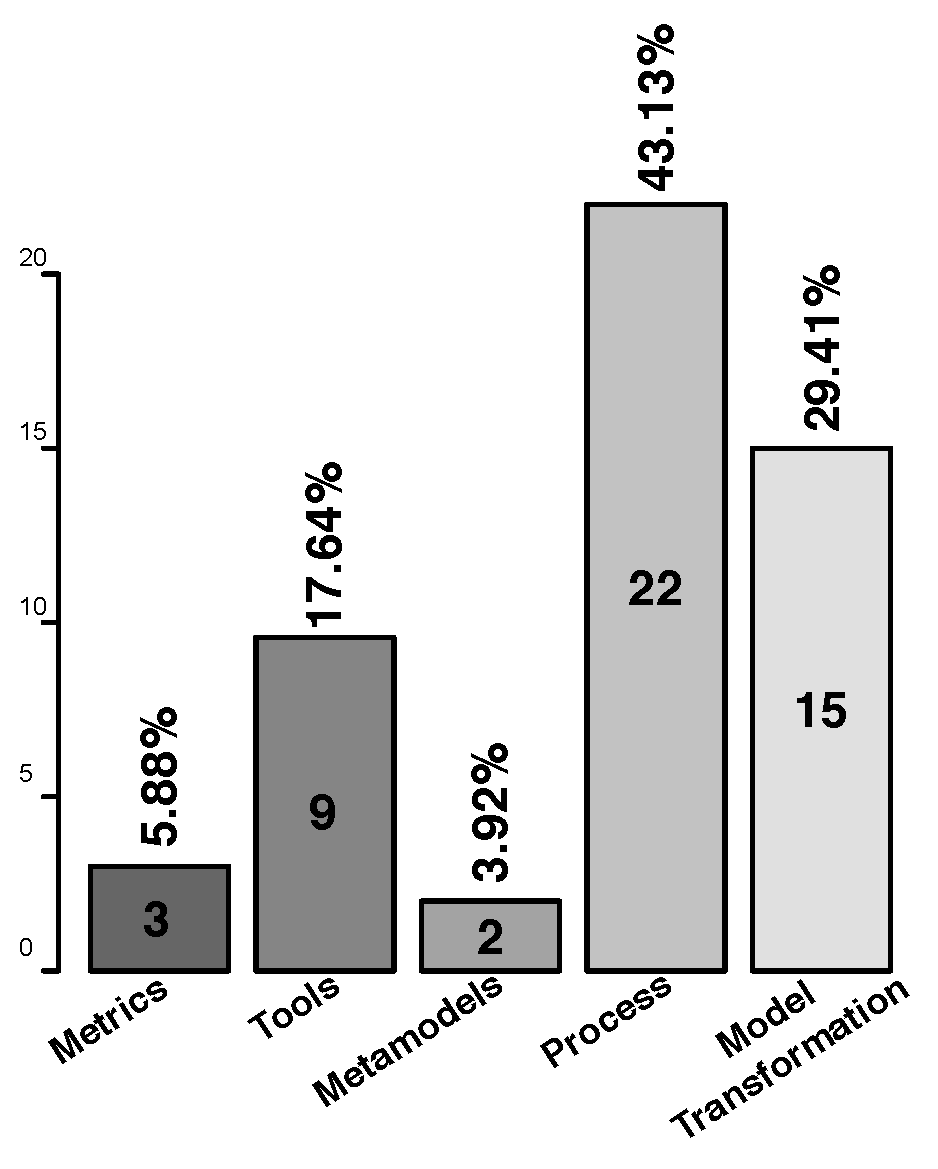
\includegraphics[width=0.2\textwidth]{figuras/NovoBarFormated}
%    }
%    \hfill
%    \subfloat[Frequency of ADM's metamodels used in literature.\label{fig:pie}]{%
%      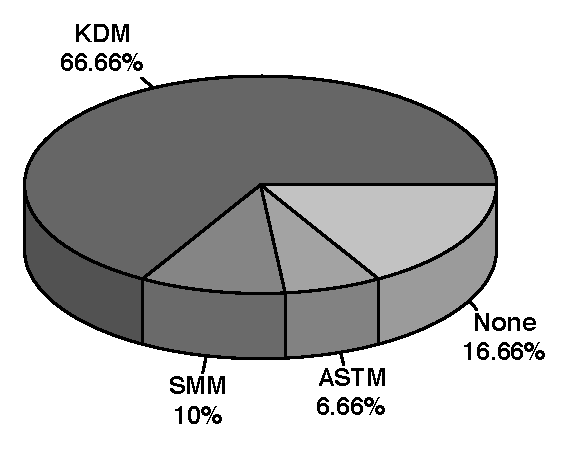
\includegraphics[width=0.2\textwidth]{figuras/pieChartModel}
%    }
%  \hfill
%    \subfloat[Frequency of research type.\label{fig:pieEvaluation}]{%
%      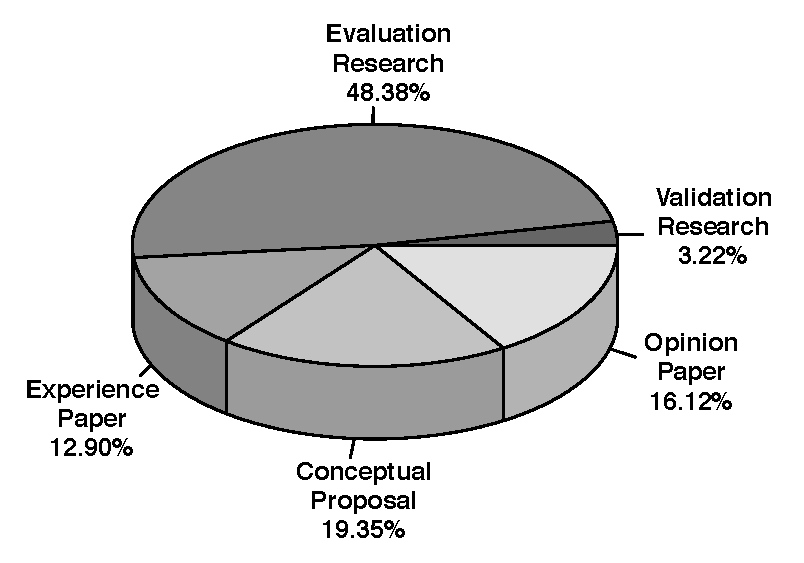
\includegraphics[width=0.25\textwidth]{figuras/pieEvaluation}
%    }
% \hfill
%    \subfloat[ADM standard metamodels used in the literature.\label{fig:pieEvaluation}]{%
%      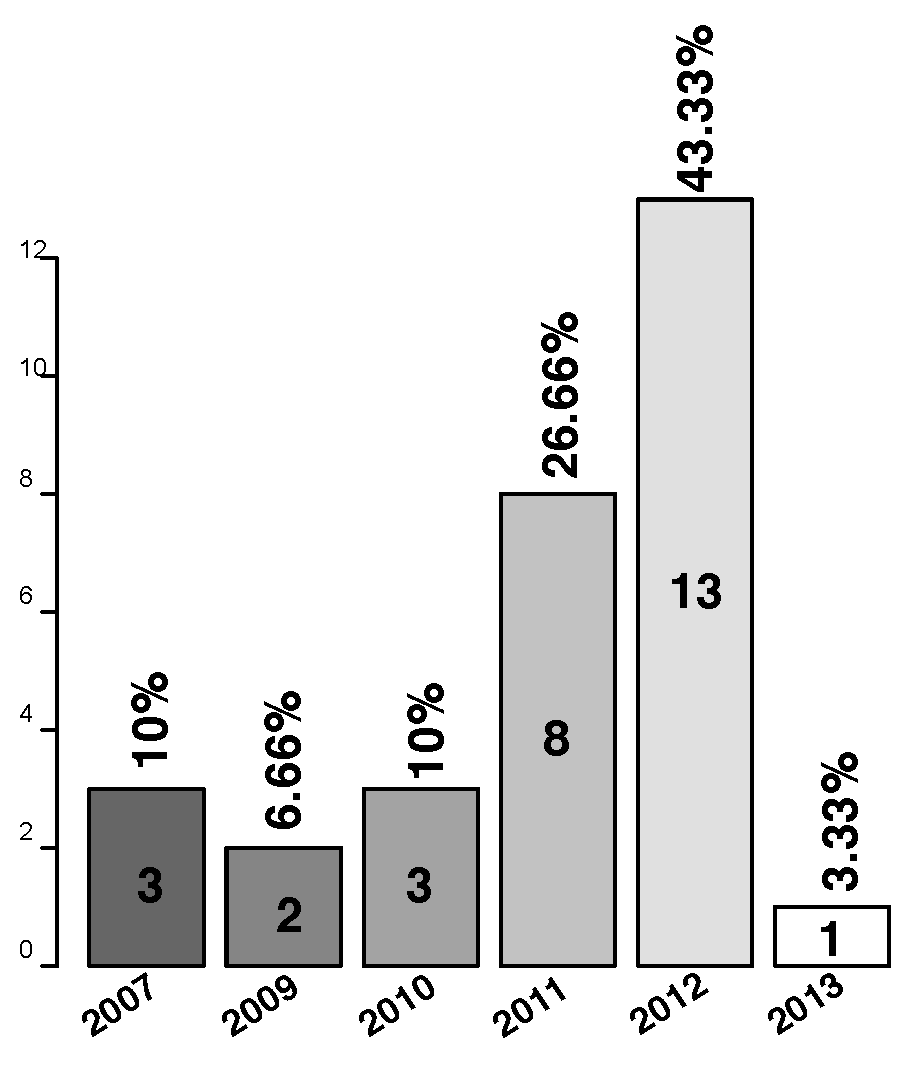
\includegraphics[width=0.2\textwidth]{figuras/DistribuicaoANoArtigos}
%    }
%    \caption{Data gathered.}
%    \label{fig:dummy}
 
% \end{figure*}

%\begin{figure}[!h]
% \centering
  % Requires \usepackage{graphicx}
%  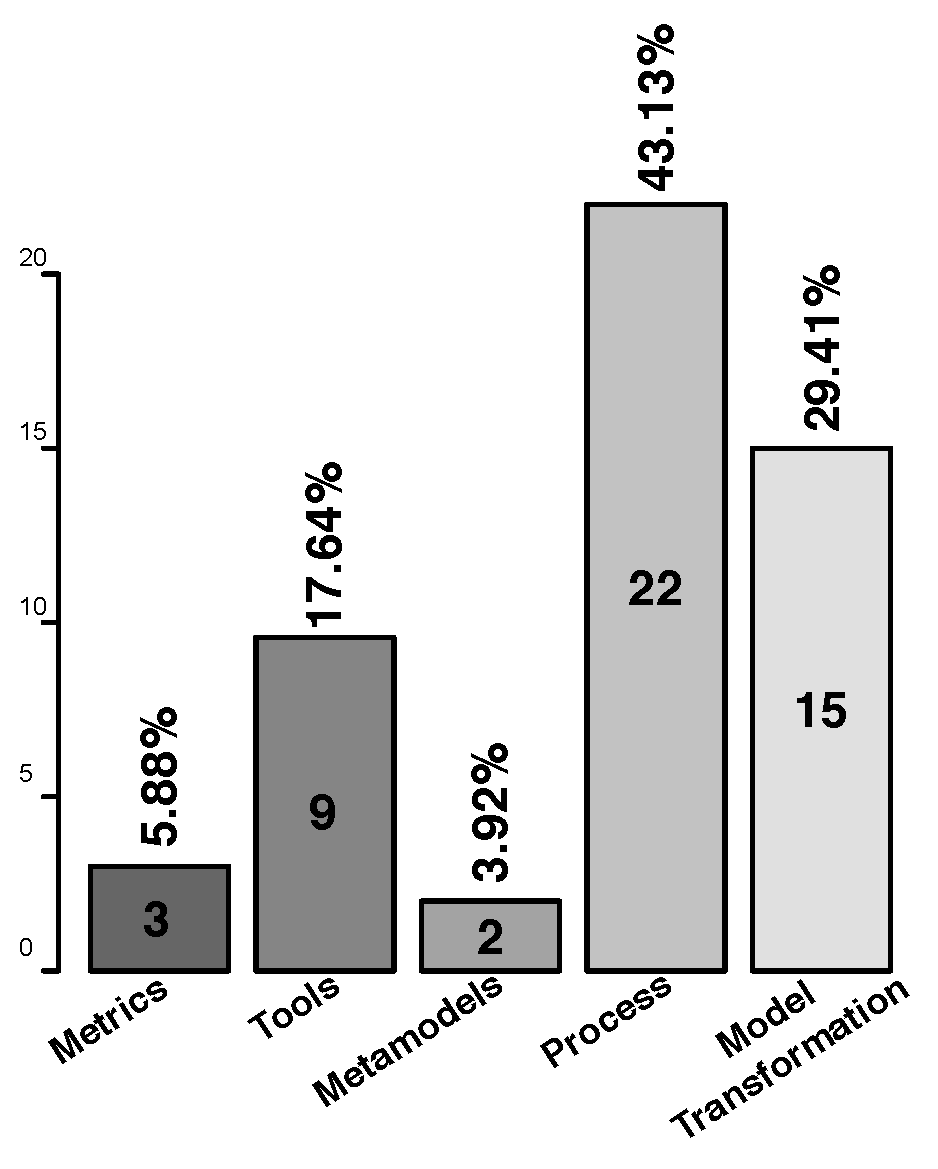
\includegraphics[scale=0.3]{figuras/NovoBarFormated}
% \caption{Frequency of studies in each category.}
% \label{fig:bar}
% \end{figure} %foi esse que eu removi, é o correto...

 As result of this analysis we answered partially the \textbf{RQ$_1$}, i.e., we answered the types of contributions that have been presented so far in liteture related to ADM and its metamodels. Another part of the \textbf{RQ$_1$}, i.e., (a discussion about the focus area regarding the ADM) has been covered in the following Sections~\ref{ssub:approach}-\ref{ssub:applicability}. We have organized each subsection in a way that it briefly describes the studies selected for each topic while highlighting the nature of research.

As for answering the first part of \textbf{RQ$_2$} we analyzed individually all identified primary studies focus on gathering which ADM standard metamodels have more been used in the literature.  In Figure~\ref{fig:pie} is depicted a pie chart wherein we have plotted the collected data. As can be seen in this figure, KDM seems to be the metamodel which has been most used in the literature, covering over 66\%. A small percentage of primary studies have reported on the use of SMM (10\%). While ASTM has been presented by rather small percentage of 6.66\%. Finally, we found out a total of 16.66\% of primary studies that does not show explicitly which metamodel has been used during the process of modernization of a legacy system. In order to answer the second part of \textbf{RQ$_2$} we gathered which are the packages most and least used within the KDM according to the identified studies. In Figure~\ref{fig:piePackage} it is fairly evident that the packages Code and Action are the most used in the literature (65\%). Maybe this came about once these packages are used to represent the source-code of system. Furthermore, the most of the studies found in the literature use somehow the source-code as input to start the modernization process. The third one most used is the Data package (15\%). This package it is used to represent relational data, such as database, XML, etc. The packages least used are Event and UI, see Figure~\ref{fig:piePackage}. 

 %\begin{figure}[!h]
 %\centering
  % Requires \usepackage{graphicx}
  % 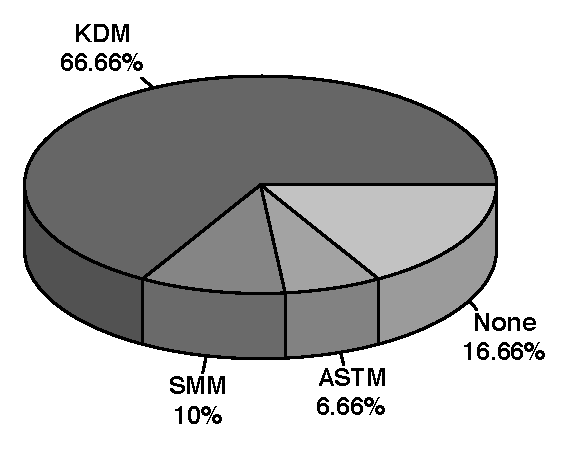
\includegraphics[scale=0.5]{figuras/pieChartModel}
 %\caption{Frequency of ADM's metamodels used in literature.}
 %\label{fig:pie}
%\end{figure} 


\begin{figure}
\def\tabularxcolumn#1{m{#1}}
\begin{tabularx}{\linewidth}{@{}cXX@{}}
%
\begin{tabular}{cc}
\subfloat[\label{fig:pie}]{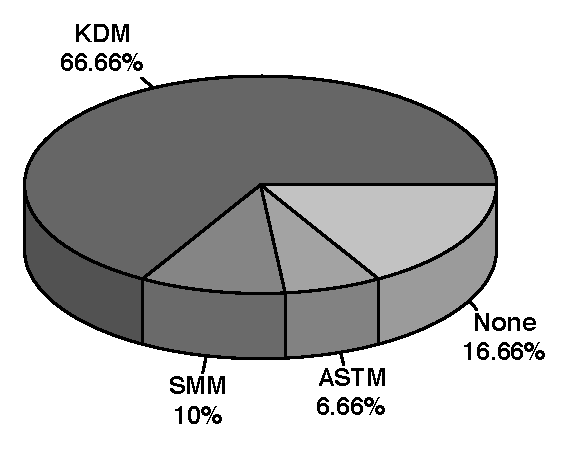
\includegraphics[width=3.9cm]{figuras/pieChartModel}} 
   & \subfloat[\label{fig:piePackage}]{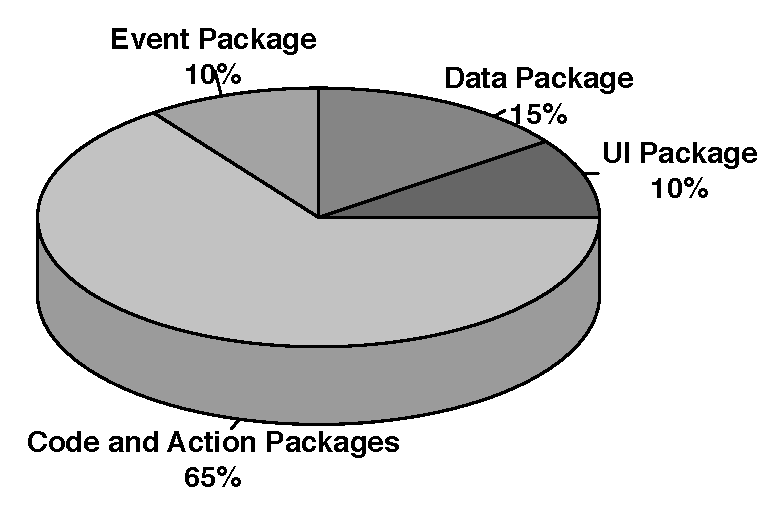
\includegraphics[width=4.5cm]{figuras/PackagesKDMFormatted}}\\
\end{tabular}
\end{tabularx}

\caption{Frequency of ADM's metamodels used in literature and packages most and least used.}\label{foo}
\end{figure}


In Figure~\ref{map}, on the facet \textbf{Research Type}, shows the data we gathered related to the research type employed in the field of ADM (\textbf{RQ$_3$}). As far as the research type is concerned, \textbf{Evaluation Research} are in vast majority, covering 15 primary stydies, see Figure~\ref{map} on the right side. A small number of publications have reported on \textbf{Validation Research} and \textbf{Experience Paper}, i.e., 1 and 4, respectively. While \textbf{Conceptual Proposal}
 and \textbf{Opinion Paper} have been presented collectively by rather of 11 primary studies.

 %Aiming to answer \textbf{RQ$_4$} we collected the name of the conference, name of the journal and the name of the workshop which the primary studies were published, Table~\ref{tab:avenue} covers the second dimension of our results and shows all avenues identified during the conducting of this review. It is fairly evident from observing the Table~\ref{tab:avenue} that the majority of primary studies were published in conference. Therefore, as result the majority of the data related to the systematic review herein were extracted from conference, i.e., among the identified primary studies (30) 23, i.e., 76.66\% studies were published in conference. Even though research has appeared on different conference we can see that in Table~\ref{tab:avenue} that we found out six journals during the review, which represent 20\%, i.e., 6 of the primary studies identified and gathered. The table also reveals that there is only one publication related to ADM and its metamodels that has appeared in a workshop so far.


\begin{figure}
\def\tabularxcolumn#1{m{#1}}
\begin{tabularx}{\linewidth}{@{}cXX@{}}
%
\begin{tabular}{cc}
\subfloat[\label{fig:bar}]{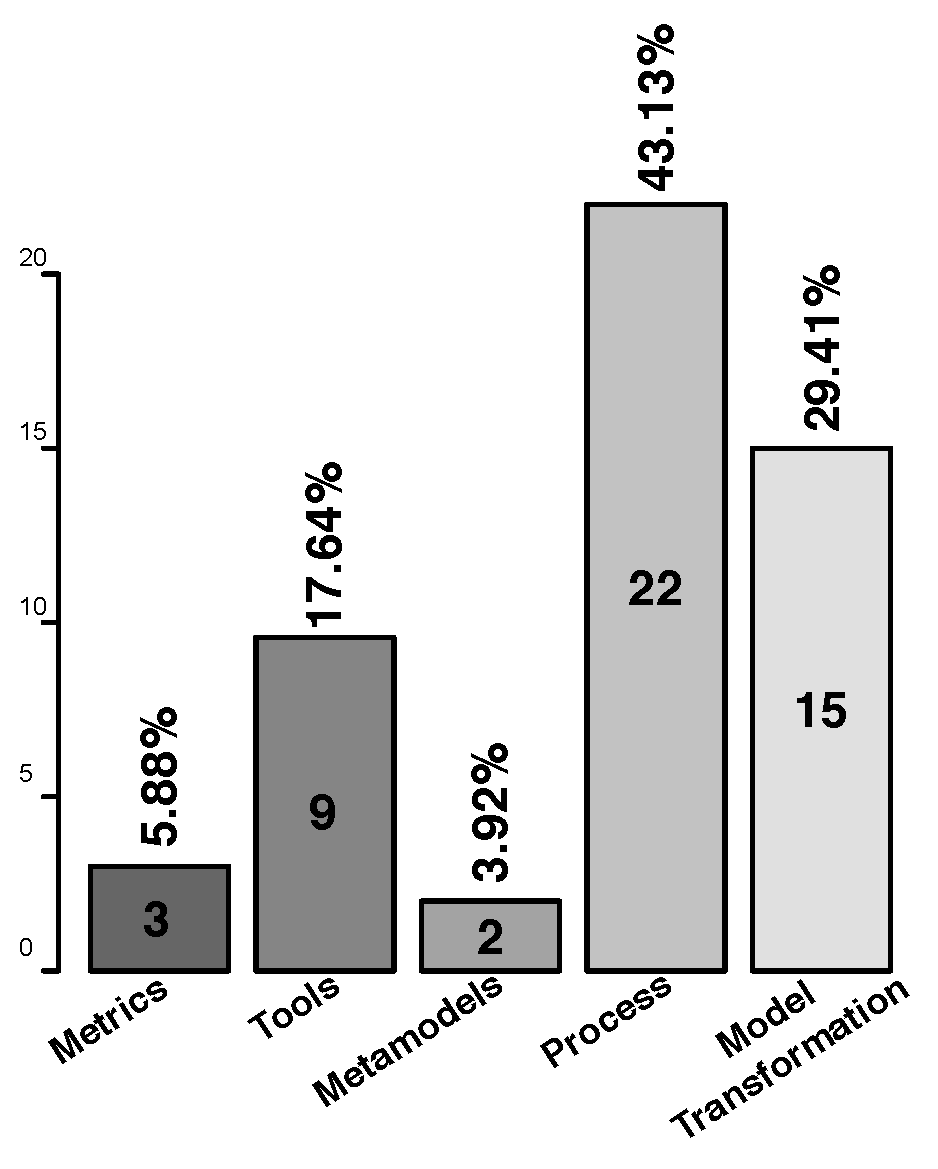
\includegraphics[width=3.9cm]{figuras/TESTEVAI}} 
   & \subfloat[\label{fig:distribuicao_de_artigo_por_ano}]{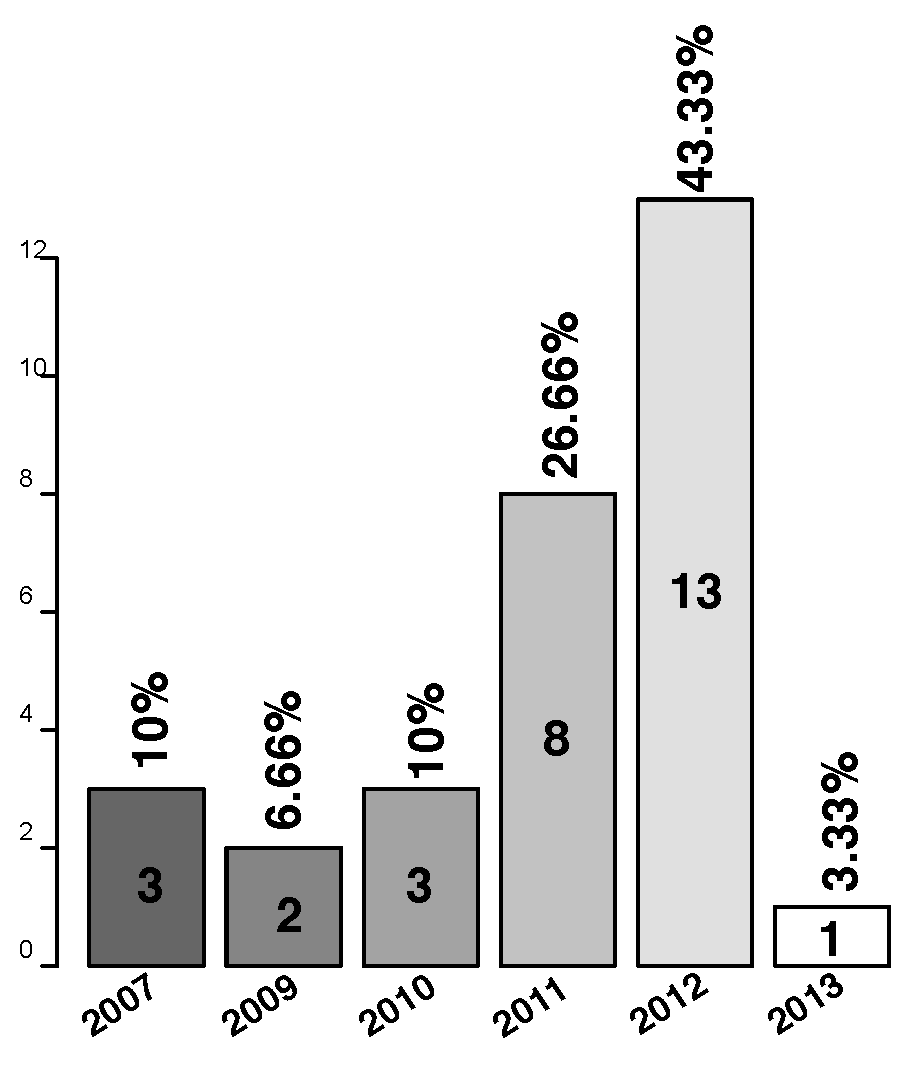
\includegraphics[width=4.2cm]{figuras/DistribuicaoANoArtigos}}\\
\end{tabular}
\end{tabularx}

\caption{Frequency of studies in each category and Distribution of publication by years. }\label{foo}
\end{figure}

 %\begin{figure}[!h]
 %\centering
  % Requires \usepackage{graphicx}
 %  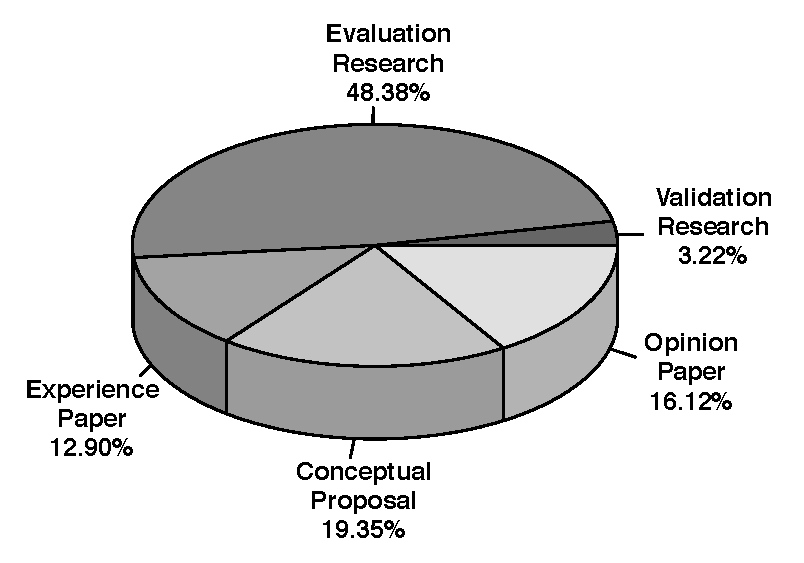
\includegraphics[scale=0.45]{figuras/pieEvaluation}
 %\caption{Frequency of research type.}
% \label{fig:pieEvaluation}
%\end{figure} 



%18 mining techniques for crosscutting concerns, as result we have answered the first part of the RQ$_1$. Based upon this bubble plot, we argue that the answer to second part of the RQ$_1$ is that Fan-In Analysis, Identifier Analysis and Dynamic Analysis are the techniques most used and Program Analysis Based, XScan-Concern-Peers, Data-Flow and Model Driven are the least used. More precisely, among the 62 primary studies included herein, 27 describe Fan-In Analysis, Identifier Analysis or Dynamic Analysis, respectively. In other hands, the techniques with less studies available in literature are Program Analysis Based, XScan-Concern-Peers, Data-Flow and Model Driven. Furthermore, it is argued that Fan-In Analysis, Identifier Analysis and Dynamic Analysis are evidence clusters (i.e., where there may be scope for more complete literature reviews to be undertaken). In contrast, Program Analysis Based, XScan-Concern-Peers, Data-Flow and Model Driven can be deemed as ``evidence desert'' (i.e., wherein better or new research is required). 





%

Finally, in Figure~\ref{fig:distribuicao_de_artigo_por_ano} shows the distribution by year of the accepted primary studies. As can be seen, the year 2012 had the biggest number of publications related to ADM and its metamodels, i.e., 43.33\%. Among the 30 primary studies included herein 8 were published in 2011, i.e., 26.66\%. In 2007 and also in 2010 were published 3 primary studies related to ADM and its metamodelo, representing 20\% of all primary studies. Among the 30 primary studies any of them were published in 2008. In 2009 was identified a percentage of 6.66 of primary studies related to the review herein. Taking into account the search strings was applied in 2013, it may explain the low amount of primary studies published in 2013. 

 %\begin{figure}[!h]
 %\centering
  % Requires \usepackage{graphicx}
  % 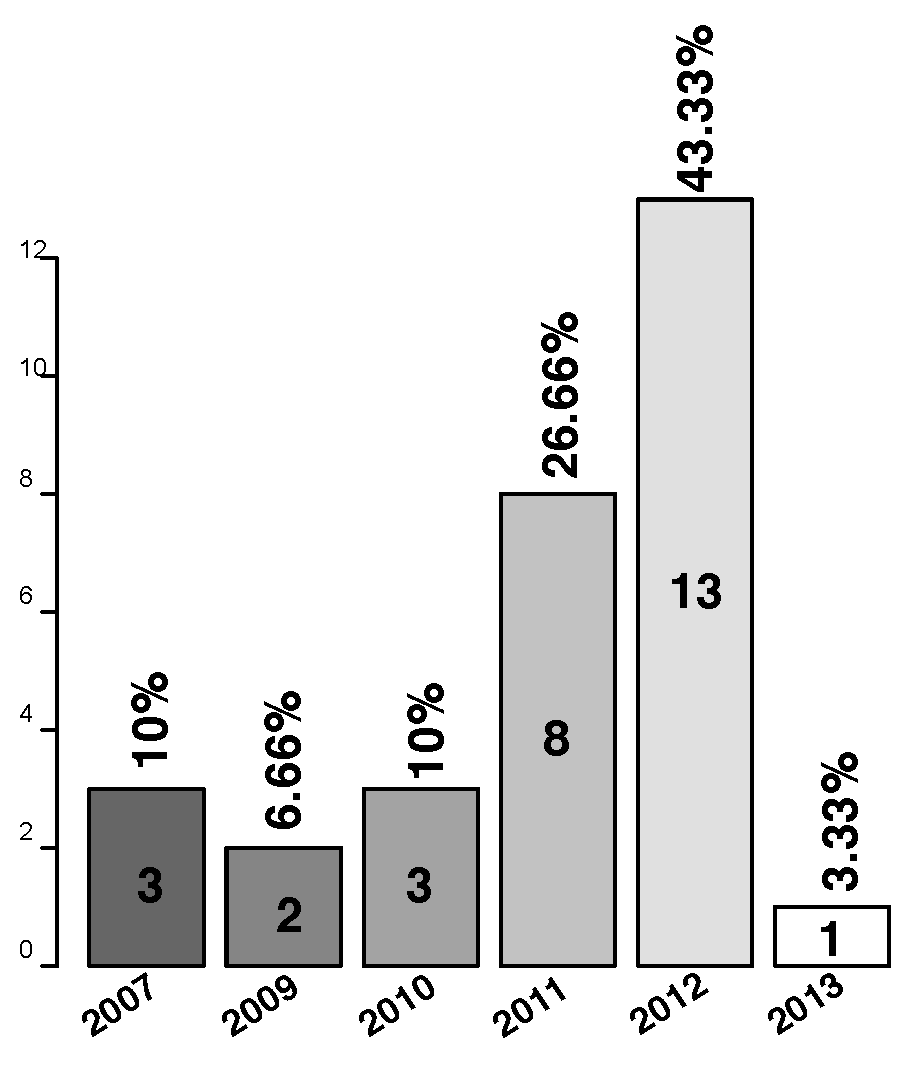
\includegraphics[scale=0.35]{figuras/DistribuicaoANoArtigos}
 %\caption{Distribution of publication by years.}
% \label{fig:distribuicao_de_artigo_por_ano}
%\end{figure} % esse é o correto 


As depicted in second bar of the Figure~\ref{fig:bar}, we identified 9 tools to assist the modernization of legacy systems. In Table~\ref{tab:tools} such tools are named and referenced. By using this table was possible to  answer the fisrt part of the \textbf{RQ$_5$}. As for answering the second part of it, a brief description about the identified tools is presented as follows. 


%As for answering the first part of \textbf{RQ$_5$}

\begin{table}
\scriptsize
\centering
\caption{The analyzed information of each tool.}
  \begin{tabular}{|l|l|l|}
\hline 
\cellcolor{gray}Name & \cellcolor{gray}Ref & \cellcolor{gray}Website\tabularnewline
\hline 
\hline 
CloudMIG &\cite{SMR:SMR582}  & tinyurl.com/cloudmigxpress\tabularnewline
\hline 
COMO &\cite{5773392}  & No\tabularnewline
\hline 
Gra2MoL &\cite{5440163}  & modelum.es/trac/gra2mol/\tabularnewline
\hline 
MARBLE &\cite{Perez-Castillo:2011:ECS:1982185.1982249,6080834, 6498507,Perez-Castillo:2010:IBP:1875847.1875861,5871783}  & No\tabularnewline
\hline 
MIMOS &~\cite{6498507} & No\tabularnewline
\hline 
MoDisco &~\cite{Bruneliere:2010:MGE:1858996.1859032} & eclipse.org/MoDisco/\tabularnewline
\hline 
PRECISO &~\cite{delCastillo:2009:PRP:1529282.1529753}  & No\tabularnewline
\hline 
R2SOA &~\cite{Guzman:2007:AAR:1339262.1339532} & No\tabularnewline
\hline 
WA2RIA &~\cite{Rodriguez-Echeverria:2011:MLW:2186508.2186536}  & No\tabularnewline
\hline 
\end{tabular}
\label{tab:tools}
\end{table}



\textbf{CloudMIG}. CloudMIG provides a semi-automatically support for the migration of software systems to PaaS or IaaS-based clouds by using KDM. This tools identifies the possible services by applying a set of rules heuristics., such as: Distribute the five most frequently used services to own virtual machines or The server methods responsible for at least 10\% of overall consumption of the CPU time shall be moved to client side components if they do not need access to the database. After, CloudMIG can generate considerable parts of a resource-efficient target architecture utilizing these rules heuristics~\cite{SMR:SMR582}. 

\textbf{COMO}. COMO provides an extension to KDM with the concepts of component and interface. By lifting the abstraction level, COMO can produce an adequate view of the entire system, and leverage the boundaries between components to better focus the subsequent modernization effort~\cite{5773392}. This tool neither offer a semi-automatically or automatically way to identify the components, i.e., the engineer has to identify the components.

\textbf{Gra2MoL}. Gra2MoL has been specifically designed to address the problem of extracting models from source code. Gra2MoL is a rule-based transformation language like existing model-to-model transformation languages, but with the fundamental difference that the source element of a rule is a grammar element instead of a source metamodel element~\cite{5440163}. Gra2MoL uses parsers to identify and to extract models from source code.

\textbf{MARBLE}. MARBLE is a modernization tool to recover business processes from legacy systems based on KDM. It uses two process mining techniques, static and dynamic analysis of source code to identify business processes. The static one is based on a module that analyze the source code file (Java files in particular) and builds an abstract syntax tree of the source code and then create an instance of KDM. On the other hand, the dynamic one takes the information about the system execution into account to extract meaningful business knowledge.

\textbf{MIMOS}. Similar to MARBLE, MIMOS also is a tool to recover business processes from legacy systems based on KDM~\cite{6498507}. This tool uses parser to identify the business processes, then a set of refactoring techniques is applied to KDM.

\textbf{MoDisco}. The goal of MoDisco is to offer an open source generic and extensible MDRE framework, as shown by Figure 2. Considering as inputs all kinds of possible legacy artifact (e.g. source code, databases, configuration files, documentation, etc), MoDisco aims at providing the required capabilities for creating models and allowing there handling, analysis and computation. As outputs, the framework targets the production of different types of artifact depending on the selected reverse engineering objective(s) (e.g. source code, data, metrics, visualizations, documentation, etc)~\cite{Bruneliere:2010:MGE:1858996.1859032}.

\textbf{PRECISO}. PRECISO is a tool for database modernisation through Web Services. Potential services can be simultaneously discovered along with database reverse engineering, i.e., a set of patterns are sought in recovered database schema~\cite{delCastillo:2009:PRP:1529282.1529753}.

\textbf{R2SOA}. This tool proposes a complete process to reengineer relational databases at a model level to integrate them into SOA contexts as a set of services. Firstly, database schema is reversed and a suitable model is built from the metadata extracted from the database catalog. Based on the structure of the database schema, a first service extraction can be undertaken, a set of model driven pattern matching is used, then CRUD operations are automatically included~\cite{Guzman:2007:AAR:1339262.1339532}.

\textbf{WA2RIA}. This tools can modernize legacy Web Applications (WA) to Rich Internet Applications (RIAs) by using ADM and KDM. This tool uses MoDisco to get an instance of KDM, then a set of rules are applied to realize the modernization of the WA to RIA~\cite{Rodriguez-Echeverria:2011:MLW:2186508.2186536}.



\subsubsection{Approach to modernize legacy systems to another platform/architecture} % (fold)
\label{ssub:approach}


In this section we briefly describes different studies regarding to propose approaches to modernize legasy systems by means of ADM.  

Jorge Maratalla et al.,~\cite{6311013} propose \textbf{GAFEMO} which aims to modernize a legacy systems to service-oriented approach taking advantage of the features provided by gap-analysis techniques. This approach takes as input a legacy system and then creates KDM representation of it. After, a set of rules are applied in this model to create the services. 


Yazdanshenas and Moonen~\cite{6080786} present a method that combines ADM with program analysis techniques to support analysis across the components of a component-based system. They build upon the foundations laid out by OMG's KDM to reverse engineer a homogeneous system-wide dependence model from a software system's heterogeneous source and configuration artifacts, and use this model as the basis for the analysis.

In~\cite{Mazon:2007:MDM:1784489.1784497} the authors propose a modernization approach for the modernization of Data warehouses following the concepts of ADM. The approach automatically performs the following tasks: (i) obtain a logical representation of data sources (\textit{ii}) mark this logical representation with MD concepts, and (\textit{iii}) derive a conceptual MD model from the marked model. 

Guzm\'{a}n and Piattini~\cite{Guzman:2007:AAR:1339262.1339532} defined an approach which is focused on the analysis of legacy systems to discover and create functionalities to be exposed as services using Web Services. The approach is based in five steps: (\textit{i}) Database reverse engineering: database schema is reversed and a suitable model is built; (\textit{ii}) First service extraction: based on the structure of the database schema, a first service extraction can be undertaken; (\textit{iii}) PIM generation: is obtained from the PSM representation using a model-to-model transformation, CRUD operations are automatically created; (\textit{iv}) Service discovering: abstract objects are identified in the PIM; (\textit{v}) WSDL generation: using the PIM, a model-to-model transformation and a WSDL (Web Service Description Language) metamodel are generated to expose the services discovered and created in the PIM and the PSM.

Frey and Hasselbring~\cite{5741334, SMR:SMR582} propose an approach based on ADM named CloudMIG that aims at supporting SaaS (Software as a Service) providers to semi-automatically migrate legacy software systems to the cloud. It is composed of six major steps: (\textit{i}) Extraction: Includes the extraction of architectural and utilization models of the legacy system, the approach uses KDM; (\textit{ii}) Selection: Selection of an appropriate CEM-compatible cloud profile candidate; (\textit{iii}) Generation: Produces the target architecture and a mapping model; (\textit{iv}) Adaptation: The adaptation activity enables a reengineer to manually adjust the target architecture; (\textit{v}) Evaluation: The evaluation activity involves static analyses and a runtime simulation of the target architecture; (\textit{vi}) Transformation: The actual transformation of the existing system from the generated target architecture to the aimed cloud environment.

P\'{e}rez-Castillo et al.,~\cite{ICEISPerez:CastilloGCP12} proposes the elicitation of database schemas, a reverse engineering technique that follows the ADM process to recover a minimal relational schema from the queries embedded in the legacy source code. In~\cite{delCastillo:2009:PRP:1529282.1529753} is presented a reengineering process that uses ADM to recover and implement Web Services in automatic manner from relational databases. P\'{e}rez-Castillo et al.,~\cite{5328801} also put forward an approach to modernize legacy systems together with the legacy relational database. This approach recovers the code-to-data linkages and obtains three kinds of models according to the ADM approach: (\textit{i}) The KDM Code Model, which represents the inventory of legacy source code. It has also the points that link the SQL Sentence Models and Database Schema Models. (\textit{ii}) The SQL Sentence Model for modelling a certain SQL query that was embedded in legacy source code. (\textit{iii}) The Database Schema Model, which represents the specific database fragment derived by an SQL Sentence Model.

In~\cite{FuentesFernandez2012247} presents the XIRUP modernization methodology, which proposes a highly iterative process, structured into four phases: preliminary evaluation, understanding, building and migration. This modernization process is feature-driven, component-based, focused on the early elicitation of key information, and relies on a ADM.

Mainetti et al.,~\cite{Mainetti:2012:MMT:2364120.2364182} present an approach that allows developers to automatically modernize the client side of legacy systems. In this approach developers can refactor the User Experience (GUI) of legacy systems during the modernization journey, taking the opportunities offered by novel interaction paradigms, i.e., Rich Internet Application (RIA). Similarly, in~\cite{Rodriguez-Echeverria:2011:MLW:2186508.2186536} the authors present an approach for the definition of a systematic process for Web Applications (WA) to Rich Internet Application (RIA) modernization, by applying ADM principles, techniques and tools. The appoach presented by the authors consists on generating a RIA client from the legacy WA presentation and navigation layers and its corresponding service-oriented connection layer with the underlying business logic at server side.

In~\cite{4400179} the authors propose an approach that uses ADM which is focused on the analysis of legacy systems to discover and create functionalities to be exposed as services using Web Services. Boussaidi et al.,~\cite{6385130} propose an approach that makes use of the KDM to reconstruct and document software architectural views of the legacy system. They consider an architectural view to be a way of partitioning a system using a specific set of KDM relevant concepts and relations and they propose clustering algorithms that target specific views mainly a layered view that we call horizontal view and a feature based view that we call vertical view. In~\cite{5440163} ADM is used into practice by building a modernization tool to generate metric reports of legacy Oracle Forms applications to assess migration efforts. The authors devised an extractor that generates KDM models from PL-SQL code (PL/SQL-to-KDM) and a metrics report generator for these KDM models. 

\subsubsection{Business Knowledge Extraction}
\label{ssub:Business_Knowledge_Extraction}

Several papers have contributed to propose approaches to identify Business Knowledge by means of ADM. A brief description of these paper are follows.

P\'{e}rez-Castillo et al.,~\cite{Perez-Castillo:2011:ECS:1982185.1982249,6080834, 6498507,Perez-Castillo:2010:IBP:1875847.1875861,5871783} present MARBLE, a modernization tool to recover business processes from legacy systems, as well as two process mining techniques within MARBLE based on static, i.e., only considers legacy source code's elements from a syntactical viewpoint and dynamic analysis of source code, i.e., it considers information derived by system execution. More specifically, this approach is based on a set of transformation: (\textit{i}) transformation obtains PSM models from each legacy software artifact using a specific metamodel for each artifact, the traditional reverse engineering techniques such as static analysis, dynamic analysis, program slicing and dicing, formal concept analysis, subsystem decomposition, and so on, can be used to extract the needed knowledge; (\textit{ii}) a set of model transformations (e.g. implemented using QVT (Query/View/Transformation)) to obtain a KDM model built from the PSM models at (\textit{i}); (\textit{iii}) transformation finally obtains the current business process model, this transformation is based on a set of business patterns. In~\cite{PerezCastillo20121370} the authors report the results of a family of case studies that were performed to empirically validate MARBLE using analysis and meta-analysis techniques. The family of case studies demonstrates that the technique is feasible in terms of effectiveness and efficiency. %P\'{e}rez-Castillo et al., also provides in~\cite{} a semi-automatic technique based on dynamic analysis, combined with static analysis to instrument the source code for obtaining event log models. A set of model transformation to transform the event log into another model following the KDM to depict legacy system, concerning its runtime viewpoint, which can be used in any software modernisation project. In~\cite{Perez-Castillo:2010:IBP:1875847.1875861} P\'{e}rez-Castillo et al., explain the KDM2BPMN model transformation within MARBLE, an ADM-based framework to rebuilt business processes embedded in legacy systems in order to facilitate and improve the evolutionary maintenance.

Normantas and Vasilecas ~\cite{lastDAyOFMyLife} present an approach that facilitates software comprehension by enabling traceability of implementation of business rules and business scenarios in the software system, i.e., their approach aim to extract business specific knowledge from the knowledge about the existing software system represented within the KDM. Ropero et al.,~\cite{Fernandez-Ropero:2012:EAB:2367051.2367064} describes a set of rules to transform Mining XML (MXML) metamodel, which is common used to represent the sequence of business activities executed by an enterprise system to KDM. The authors takes an MXML model and obtains an equivalent KDM model at the same abstraction level. The proposed set of rules consist of eight declarative transformation rules. 


\subsubsection{Extension of ADM's metamodels} % (fold)
\label{ssub:extension_of_adm_s_metamodels}

We have identified two papers that address how to perform extension of ADM's metamodels. We provided a brief summary of these paper are follows. 

In~\cite{5773392} proposes the COMO (Component-Oriented MOdernization) metamodel an KDM's extension, by borrowing recurring concepts from component-based solutions and software architectures, and to support a proper componentization of the system to assist the modernization of legacy systems. In~\cite{Perez-Castillo:2012:IEL:2231936.2231949} propose an extension to the KDM that aims to represent all the information registered in a MXML model in the KDM model. They claimed that the impact of this extension on well-proven and KDM based tools is not problematic since it is carried out with the own extension mechanism of the KDM standard. Besides this fact, most elements of the event model are present in the core of KDM which is used for many tools.

% subsubsection extension_of_adm_s_metamodels (end)

\subsubsection{Applicability} % (fold)
\label{ssub:applicability}

Similarly, we also have identified a small number of papers that address just the applicability of the ADM and its metamodel. A summary of these paper are follows.

Normantas et al.,~\cite{Normantas:2012:OKD:2383276.2383286} describe all concepts related to the metamodel KDM. The authors claim that the paper enables researchers and practitioners to get a better understanding KDM. This paper also provide a reference for the researchers and practitioners that are interested in using the KDM for the purpose of modernization, and would establish a basis for the further research. 

P\'{e}rez-Castillo et al.,~\cite{PrezCastillo2011519} present how to use KDM to modernize legacy systems. Also in this paper the authors described each layer of the metamodel KDM, they also presented a set of example of how to use ADM and KDM during the modernization of a legacy systems.

% subsubsection applicability (end)









	
\section{Threats to Validity}\label{threats}
		\textbf{Primary studies selection}. Aiming at ensuring an unbiased selection process, we defined research questions in advance and devised inclusion and exclusion criteria we believe are detailed enough to provide an assessment of how the final set of primary studies was obtained. However, we cannot rule out threats from a quality assessment perspective, we simply selected studies without assigning any scores. In addition, we wanted to be as inclusive as possible, thus no limits were placed on date of publication and we avoided imposing many restrictions on primary study selection since we wanted a broad overview of the research area.

\textbf{Missing important primary studies}. The search for primary studies was conducted in several search engines, even though it is rather possible we have missed some primary studies. Nevertheless, this threat was mitigated by selecting search engines which have been regarded as the most relevant scientific sources~\cite{Dyba} and therefore prone to contain the majority of the important studies.

\textbf{Reviewers reliability}. All the reviewers of this study are researchers in the software reuse field, focused on software testing and software product line, and none of the approaches and tools developed by us. Therefore, we are not aware of any bias we may have introduced during the analyses.

\textbf{Data extraction}. Another threat for this review refers to how the data were extracted from the digital libraries, since not all the information was obvious to answer the questions and some data had to be interpreted. Therefore, in order to ensure the validity, multiple sources of data were analyzed, i.e. papers, technical reports, white papers. Furthermore, in the event of a disagreement between the two primary reviewers, a third reviewer acted as an arbitrator to ensure full agreement was reached.
		
%\section{Related Work}\label{related}
%	Closely related work to this review is a survey with aspect mining techniques \cite{Kellens}, which details and compares a large selection of automated techniques and aspect mining tools. The goal is to present a comparative framework for distinguishing aspect mining techniques, and assess known techniques against this framework. 
			
\section{Concluding Remarks}\label{conclusion}
		Our long-term research goal is to find out how ADM has been applied in the literature to assist engineers during the process of modernization of legacy system. To do so in this paper we presented a systematic review of ADM and its metamodels, following the process described by Kitchenham~\cite{Dyba}. Through a examination of 30 primary studies encompassing ADM, this review has presented 22 papers which describe processes, 15 that propose a set of model transformation, 9 that put forward tools, 3 which present metrics and 2 that illustrate same extension in the ADM's metamodels. Notice that certain primary studies were grouped in more than one category, affecting the frequency count; i.e., the sum of the frequencies shown in each facet of the Figure~\ref{map} can be greater than the total of selected studies identified, i.e., 30. We claim that researchers can use this review as a basis for advancing the field, while practitioners can use it to identify process, tools, metrics, etc that are well-suited to their needs. This systematic review should serve not only academic researchers but also industrial professionals, aiming at adopting some process, tool, metrics, to modernize a legacy systems within their organizations. %The review described in this paper reveals that the most mentioned mining techniques for crosscutting concern are Fan-In Analysis, Identifier Analysis and Dynamic Analysis. In contrast, Program Analysis Based, XScan-Concern-Peers, Data-Flow and Model Driven can be deemed as  ``evidence desert''. 

The initial significant contributions to ADM were presented in 2007 (i.e.,~\cite{Mazon:2007:MDM:1784489.1784497, Guzman:2007:AAR:1339262.1339532, 4400179}), in 2008 had no publications. However, in 2009 we identified two paper dealing with ADM (i.e.,~\cite{delCastillo:2009:PRP:1529282.1529753, 5328801}). Next, we had a rise from 2010 (3 papers) to 2011 (8 papers). After, in 2012  
the rate of papers gradually rose to 13. Then, it dropped out in 2013. This may happed once we carried out the review in 2013. Among these paper were found that most of them have appeared in conferences and journal, while just a was reported in workshop.

In summary, this review shows that there are some researchers investigating related to ADM and its metamodels. As consequence, we were able to identify that there are a set of process which have been commonly used in literature to assist the software engineer to modernize legacy system by means of ADM. Afterwards, was also possible to identify that KDM is the ADM's metamodel more utilized into the literature. Similarly, the KDM's packages most used in the literature are Code and Action - the least used are Event and UI packages.

 As future work, other related systematic review are about to be concluded and the relationship among their results should be investigated aiming to characterise this area in a deeper way. As soon as they are concluded, their results should be presented for the academic community as a technical report that will become available online.





%Research in the area of aspect-oriented modeling and model- driven code generation can result in significant advancement in development of software systems that are more maintainable, extensible and reusable. To get an overall view of the current re- search in this area, we defined a few research questions and launched a systematic mapping study. We found 65 publications that possess maximum relevance to fulfill objectives of our study. The selected papers have appeared between 2002 and 2011.
%The results of this study indicate that aspect-oriented modeling and code generation is a rather underdeveloped area. The initial significant contributions to this area were presented in 2002 (i.e. [55,56]), most papers have appeared in workshops and confer- ences, while a few were reported in journals.



%Based on the identified techniques we have extended the taxonomy proposed by Kellens et al.~\cite{Kellens}. This new taxonomy contains 7 new  mining techniques for crosscutting concerns. By using this taxonomy we hold that this taxonomy could serve as an initial roadmap to crosscutting concern researchers. Moreover, this extended taxonomy could be relevant for tool developers who might have knowledge about the best aspect indicators to use or who may have certain demands about the granularity of the results.

%The main future directions that emerged from this review are the need for empirical, comparative evaluations and the opportunity for developing combined techniques. Indeed, since every technique relies on different assumptions and uses different underlying analysis techniques, the found techniques are highly complementary, which suggests the possibility of several useful combinations. Thus, through the results obtained in this review we argue that if one pretends to devise a new mining techniques for crosscutting concerns to mine either Persistence or Observer, a good initial point is to take into consideration the combination herein illustrated in Table~\ref{table_conclusion} and~\ref{table_conclusion2} but more studies are needed because the combinations proposed did not take into consideration the versions of the system, so we intend to analyze this in future works.


% that could improve precision and recall metrics.Thus, if new mining techniques are developed then software engineers must test a wide range of concerns taking into account implementation variabilities. Finally, through the results obtained in this review we argue that if one pretends to devise a new mining techniques for crosscutting concerns to mine either Persistence or Observer, a good initial point is to take into consideration the combination herein illustrated in Table~\ref{table_conclusion} and~\ref{table_conclusion2}.


%We learned from this review that it is important to perform studies showing the pros and cons of using combinations of several mining techniques for crosscutting concern in a unique software environment. One type of analysis that can be performed is to combine techniques with high values of recall and high values of precision. Although the Table~\ref{table_conclusion} shows one tool (CBFA) using combined techniques, we can not  infer whether or not the tool has improved their capability to identify crosscutting concerns because we do not have the precision and recall metrics for each tool acting separately with the same conditions and one example is not representative. However, it could be a strategy for searching new techniques, i.e., combining CBFA with XScan. The idea behind this type of combination is to mitigate deficiencies in the way they do the identification of concerns because most probably one group of techniques is better adapted to find out a sort of concerns while others may have better results on others. Furthermore, it could be interesting to try to classify techniques according to the domain in which they act, i.e., non-functional and functional concerns. The Dynamo tool has a good precision for Persistence concern but not so good for Undo. Similarly, CBFA has a high value of precision for Undo and low value of precision for Persistence. Nevertheless, more studies are needed to confirm if Dynamo is most suitable for non-functional concern and future research might resolved this issue. We have presented candidate combinations of techniques that could improve precision and recall metrics. The comparison allowed us to show that the precision and recall can change quite a lot, when concern is different. Thus, if new mining techniques are developed then software engineers must test a wide range of concerns taking into account implementation variabilities. Finally, through the results obtained in this review we argue that if one pretends to devise a new mining techniques for crosscutting concerns to mine either Persistence or Observer, a good initial point is to take into consideration the combination herein illustrated in Table~\ref{table_conclusion} and~\ref{table_conclusion2}.

%\section{ACKNOWLEDGMENTS}\label{ack}
%	      Rafael Durelli would like to thank the financial support provided by FAPESP, process number 2012/05168-4. Daniel Santib\'a\~nez would like to thank the financial support provide by CAPES. Valter Camargo would like to thank CNPQ, process number 560241/2010-0. We also thank Thiago Gottardi for his proofreading of this paper.
	
%References
\bibliographystyle{abbrv}		
\bibliography{acmSac2013}


\end{document}
